% !TeX program = xelatex
\documentclass{article}

% Copy of the official ICLR 2027 style; the original template is unchanged.
\usepackage{iclr2027_conference,times}
\input{math_commands.tex}

% English XeLaTeX configuration.
\usepackage{fontspec}
\IfFontExistsTF{TeX Gyre Termes}{\setmainfont{TeX Gyre Termes}}{\setmainfont{Times New Roman}}
\IfFontExistsTF{TeX Gyre Heros}{\setsansfont{TeX Gyre Heros}}{\setsansfont{Arial}}

\usepackage{graphicx}
\usepackage{wrapfig}
\usepackage{float}
\usepackage{booktabs}
\usepackage{array}
\usepackage{tabularx}
\usepackage{multirow}
\usepackage{amssymb}
\usepackage{xcolor}
\usepackage{hyperref}
\usepackage{url}

\graphicspath{{figures/}}
\hypersetup{unicode=true,colorlinks=true,citecolor=blue,linkcolor=blue,urlcolor=blue}
\newcommand{\cmark}{\ensuremath{\checkmark}}
\newcommand{\xmark}{\ensuremath{\times}}
\definecolor{tablegreen}{RGB}{0,139,139}
\definecolor{tablered}{RGB}{220,50,47}
\newcommand{\cmarkcolor}{\textcolor{tablegreen}{\cmark}}
\newcommand{\xmarkcolor}{\textcolor{tablered}{\xmark}}
\newcommand{\methodname}{GroundedHuman}
\newcommand{\todoresult}{\textcolor{tablered}{To be evaluated}}
\newcommand{\placeholdernote}[1]{\textcolor{tablered}{\textbf{Placeholder: #1}}}

\title{GroundedHuman: Metric 4D Human-Scene Reconstruction with Geometric Interaction Learning}

% ICLR 2027 double-blind submission: keep \iclrfinalcopy commented.
\author{Anonymous Authors}
%\iclrfinalcopy

\begin{document}
\maketitle

\begin{figure}[h]
\centering
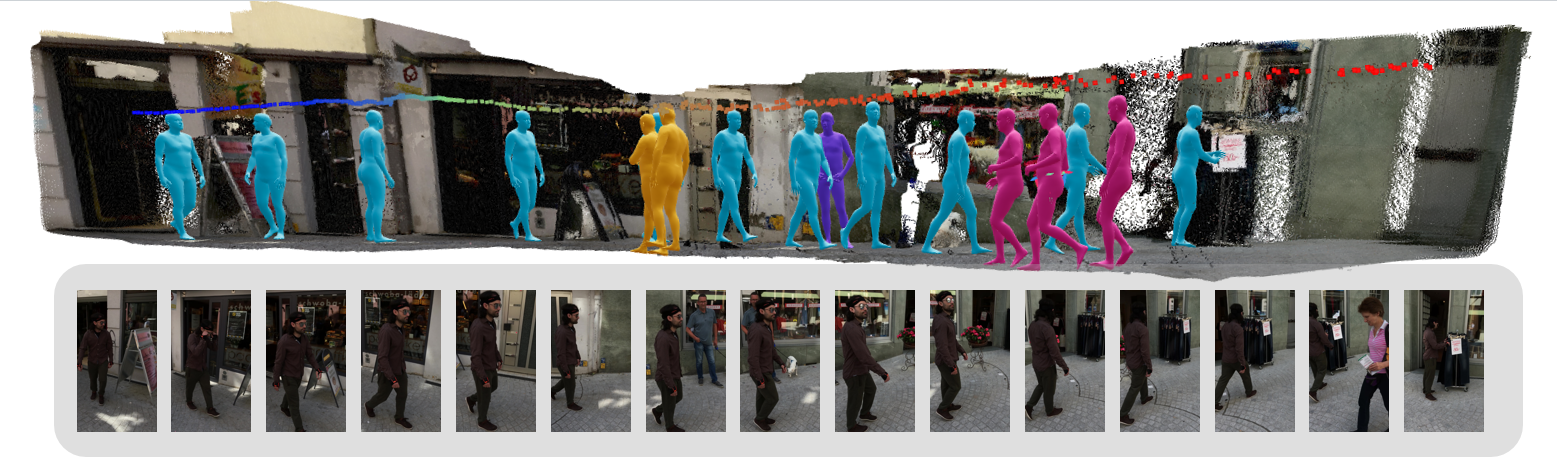
\includegraphics[width=\textwidth,height=2.15in,keepaspectratio]{figures/fig1_teaser_real.png}
\caption{Temporal human--scene reconstruction produced by GroundedHuman. The top row shows the accumulated metric scene, time-coded human meshes, and camera trajectory in a shared world coordinate system; the bottom row shows the corresponding input video frames. Humans, scene geometry, and camera motion are jointly visualized under the same scale and coordinate gauge.}
\label{fig:teaser}
\end{figure}

\begin{abstract}

We present GroundedHuman, a geometric interaction learning framework for recovering a scale-consistent 4D human--scene world from casually captured monocular videos. Existing methods can already jointly predict scenes, cameras, and humans, but joint outputs do not inherently guarantee metric consistency: the relative geometry recovered by scene foundation models and the metric scale encoded by parametric human bodies may still reside in different coordinate gauges, thereby corrupting camera trajectories, world-space human motion, and human--environment relationships. Our central insight is that a human should be viewed not only as a dynamic reconstruction target in the scene, but also as an intrinsic metric anchor connecting scene geometry, camera motion, and human trajectories. Based on this insight, GroundedHuman constructs a human-scale bridge that establishes robust scene-scale consensus from visible human surfaces and uses person-conditioned residual calibration to consistently propagate the same metric gauge to scene depth and camera translation. Building on this calibrated geometry, we further introduce TRSTR, which extracts local geometric interaction evidence from canonical body regions and their surrounding environment, and refines world-space human positions through constrained, confidence-aware iterative updates while strictly preserving the existing local pose and shape. In this way, GroundedHuman unifies relative scene geometry, camera trajectories, and multi-person motion within a single physically meaningful 4D world. Extensive experiments demonstrate that the framework significantly improves world-coordinate human motion while retaining strong local human reconstruction performance, and exhibits stable metric reconstruction capability in camera trajectory and video depth evaluations. These results validate our central claim: humans in a scene constitute a powerful and general geometric prior that can establish a shared metric coordinate gauge for visual reconstruction when reliable absolute scale is unavailable.

\end{abstract}
\section{Introduction}\label{sec:introduction}

Recovering a dynamic 3D world from casually captured monocular video is a basic capability for embodied intelligence, augmented reality, robotic perception, and human behavior understanding. A complete world model must reconstruct not only the static environment, but also camera motion and the poses and trajectories of one or more people, all expressed in a common world coordinate system \citep{chen2026human3r,li2026unish,liu2026josh}. Although this appears to be a simple combination of scene reconstruction and human mesh recovery, it imposes a stricter metric requirement: scene depth, camera translation, and human position must share a physical scale. Otherwise, locally plausible geometry still produces incorrect camera baselines, human world trajectories, and human--environment relationships.

Learning-based 3D reconstruction and human mesh recovery have progressed rapidly along largely separate tracks. DUSt3R, MASt3R, and their dynamic extensions establish cross-view 3D correspondences with pixel-aligned pointmaps \citep{wang2024dust3r,leroy2024mast3r,zhang2024monst3r}; CUT3R, VGGT, $\pi^3$, and VGGT-Ω further strengthen scene and camera reasoning for multi-view images and videos \citep{wang2025cut3r,wang2025vggt,wang2025pi3,wang2026vggtomega}. In parallel, SMPL/SMPL-X-based HMR models recover stable local humans from challenging images and videos, while TRAM, WHAM, GVHMR, and DuoMo lift human motion to world coordinates \citep{wang2024tram,shin2024wham,shen2024gvhmr,wang2026duomo}. These advances provide strong scene structure and human priors, but do not automatically place both outputs in the same metric gauge: relative depth and camera translation can be jointly rescaled without changing image projections, and world-space human motion directly inherits this unresolved scale.

Recent joint human--scene methods have begun to connect these two priors explicitly. JOSH obtains geometrically consistent reconstructions by jointly optimizing camera, scene, human, and contact constraints at test time, while JOSH3R distills the result into a learned predictor \citep{liu2026josh}; Human3R and UniSH jointly read out scenes, cameras, and humans through human prompts or AlignNet \citep{chen2026human3r,li2026unish}; UniCon3R further uses contact as an internal correction signal \citep{sur2026unicon3r}. These methods improve consistency through joint representations, contact, or human placement. The closest related approaches are MetricHMSR, which uses a metric human to guide per-pixel affine depth correction in a single image, and GRAFT, which iteratively updates human pose, shape, translation, and scale using local geometry probes in an external metric scene \citep{song2026metrichmsr,ym2026graft}. However, a clear decomposition is still missing for using a metric human in video to fix the scale gauge of a relative scene and camera while refining world position without changing local human pose.

Our starting point is simple: a person is not only a dynamic object to reconstruct, but also one of the few scene elements with predictable physical dimensions. The SMPL meshes produced by NLF are already expressed in meters \citep{sarandi2024nlf,loper2023smpl}; when human projection, scene depth, and camera intrinsics share the same image plane, the ratio between the visible human-surface Z-depth and the relative depth at the same pixels provides a scale constraint. The challenge is that this constraint is not uniformly reliable. Human initialization errors, self-occlusion, inter-person occlusion, depth boundaries, and local scene noise produce heavy-tailed ratios and incorrect correspondences. Human scale therefore cannot be reduced to a direct ratio from one joint or one depth sample; it requires constrained robust estimation over visible surfaces, multiple people, and temporal scale consistency.

Based on this observation, we build a human-scale bridge that combines analytic normalization with learned residuals. We project the SMPL surface of each confident person into the VGGT-Ω relative-depth map and use a z-buffer-like front-surface test to remove occlusion conflicts at shared pixels. The median of all valid surface ratios provides an analytic coarse scale and removes the dominant scene-scale freedom. We then use 24 body anchors as human--scene interaction tokens, query local depth residuals and multi-level VGGT-Ω scene features, and predict a near-identity residual scale and depth bias. For world reconstruction, analytic and residual scales are jointly aggregated within a clip, and the same shared scale is applied to depth and camera translation. This decomposition assigns scale magnitude to analytic geometry and leaves the learned module to model only local residuals caused by occlusion, projection, and depth bias.

Metricizing the scene does not guarantee that the human is perfectly placed relative to local surroundings. We therefore introduce TRSTR, a regional translation-refinement module. TRSTR organizes the SMPL surface into 96 regions with stable anatomical correspondence and probes self-surface, environment, and other-human geometry around each region. Each region proposes a bounded translation vote in a camera ray/tangent basis; region gates, predicted uncertainty, and a person gate then aggregate these votes into a shared root update. After every update, the human is reprojected and scene evidence is recollected, forming a two-step geometric loop. Unlike methods that jointly update all human parameters, TRSTR restricts the optimization space to camera-space translation and cannot reduce world-space error by altering pose or shape.

We evaluate this design along four dimensions: local human recovery, world-space motion, camera trajectory, and metric depth. On 3DPW, we preserve NLF's 37.3 mm PA-MPJPE, 60.3 mm MPJPE, and 71.4 mm PVE, showing that scale and translation calibration does not damage local human quality. On EMDB-2, we obtain 58.468 mm WA-MPJPE, 149.959 mm W-MPJPE, and 1.079\% RTE, indicating that the main gains arise from scale-consistent camera-to-world transformations and root trajectories. On TUM-Dynamic, VGGT-Ω maintains a 0.00692 m ATE with 500 input views, providing a stable basis for long camera trajectories. On Bonn, human-scale calibration reaches 0.08599 Abs Rel and 0.96377 $\delta<1.25$ accuracy without GT scale or shift, further showing that a human can convert stable relative structure into effective metric depth.

We summarize our contributions as follows: 1) We propose a human-anchored scale-normalization framework that turns the metric SMPL surface into an intrinsic reference for a relative scene and consistently propagates the recovered shared scale to scene depth and camera translation; 2) we design a coarse-to-fine geometric calibration process composed of visible-front-surface analytic scale estimation, person-conditioned residual affine calibration, and TRSTR, where TRSTR uses canonical anatomical regions and heteroscedastic local votes to correct only the human root translation while preserving local pose and shape; and 3) we establish an evaluation chain on 3DPW, EMDB-2, TUM-Dynamic, and Bonn that covers local human recovery, world-space motion, camera trajectories, and scene depth, verifying that humans in the environment can provide an effective metric anchor when reliable absolute scene scale is unavailable.

\section{Related Work}\label{sec:related-work}

\subsection{Learning-based 3D and 4D Scene Reconstruction}

Classical Structure-from-Motion systems use feature matching, triangulation, and bundle adjustment to recover accurate sparse geometry and camera trajectories in static scenes, with COLMAP as a representative system \citep{schonberger2016colmap}. Recent learned reconstruction systems integrate correspondence estimation, geometric recovery, and camera solving into unified networks. DUSt3R connects 3D relations between image pairs through pixel-aligned pointmaps \citep{wang2024dust3r}, while MASt3R adds dense descriptors to strengthen cross-view matching \citep{leroy2024mast3r}. MonST3R extends pointmap reconstruction to dynamic videos \citep{zhang2024monst3r}; CUT3R supports incremental 4D reconstruction through persistent state \citep{wang2025cut3r}; and VGGT and $\pi^3$ move beyond the image-pair paradigm with global multi-view reasoning \citep{wang2025vggt,wang2025pi3}.

These models improve scene coverage for uncalibrated images and dynamic videos, and allow cameras, depth, and scene features to be inferred jointly. VGGT-Ω follows this direction with camera tokens, scene registers, and dense prediction heads for multi-view camera parameters and depth, while exposing scene representations reusable by downstream tasks \citep{wang2026vggtomega}. Yet projection-consistent scene geometry can retain a global scale gauge: without a reliable metric reference, depth and camera translation can be scaled together without changing image reprojection. Existing general-purpose reconstruction work primarily optimizes scene structure and cross-view consistency, rather than studying how the canonical physical size of a person in a video can constrain this gauge.

We use the relative scene and camera from VGGT-Ω as the structural foundation, but do not introduce a new general-purpose scene backbone. Instead, we turn the SMPL body already present in the scene into an intrinsic metric anchor: the front surface analytically fixes the dominant scene scale, a person-conditioned module estimates a residual affine, and the final scale acts on both depth and camera translation. This setup separates general geometric recovery from human-driven metric normalization and directly tests whether a scene model without reliable absolute scale can recover a shared metric coordinate system from a person.

\subsection{World-space Human Motion Recovery}

Human mesh recovery has traditionally targeted pose and shape in camera coordinates. SMPL/SMPL-X optimization methods fit human parameters to 2D keypoints and silhouettes \citep{loper2023smpl,pavlakos2019smplx}, while learned HMR directly regresses local humans from image or video features \citep{chen2026human3r,song2026metrichmsr}. Local HMR now provides strong priors under challenging poses and occlusion, but a camera-space human does not directly determine a world trajectory: monocular video entangles camera motion, human motion, and depth scale, and systematic error in any component accumulates in the camera-to-world transform \citep{wang2026duomo}.

Existing world-space human methods broadly follow two routes. One first estimates a camera-space human and then lifts it to world coordinates using SLAM, camera trajectories, gravity, or external metric depth. GLAMR uses motion priors to complete occlusion and recover global trajectories \citep{yuan2022glamr}; TRAM improves SLAM scale stability with dynamic-region masks and monocular metric depth \citep{wang2024tram}; and WHAM and GVHMR introduce trajectory regression, gravity, and viewing-direction constraints \citep{shin2024wham,shen2024gvhmr}. The other route directly learns world-space human distributions. DuoMo decomposes the problem into camera-space and world-space diffusion stages and generatively denoises lifted motion proposals in each video's own world coordinate system \citep{wang2026duomo}.

The main output of these methods is global human motion; scene geometry typically serves as a camera-estimation, ground-orientation, or post-processing constraint rather than a dense reconstruction target shared with the human \citep{yuan2022glamr,wang2024tram,shin2024wham,shen2024gvhmr,wang2026duomo}. We do not introduce a new human-motion generative prior or re-estimate the local pose and shape already provided by NLF. Instead, we exploit a bidirectional scale relation between human and scene: a metric human first constrains the relative scene, and the calibrated scene and camera then provide local geometric references for human root translation. World-space accuracy is therefore improved through two variables, scale and root translation, while the local HMR path remains unchanged.

\subsection{Joint Human--Scene Reconstruction}

Joint human--scene reconstruction seeks to recover humans, cameras, and the surrounding environment in one coordinate system. Early methods typically combine scene reconstruction, HMR, contact prediction, and motion priors, then jointly optimize multiple variables at test time. JOSH starts from local humans, depth, point correspondences, and human--scene contacts, and jointly optimizes camera poses, multi-person world motion, and a dense scene; its contact term turns support relationships into an explicit constraint linking scene and motion \citep{liu2026josh}. This route directly optimizes geometric consistency, but its inference cost and sensitivity to initialization motivated later learned models such as JOSH3R that distill the optimization result \citep{liu2026josh}. For large multi-person scenes, Crowd4D further uses a Human-Scene Interaction Proxy to constrain group scale and individual world positions, and maintains consistency on complex terrain through multi-stage optimization \citep{kang2026crowd4d}.

Another line injects human awareness directly into learned scene reconstruction. HAMSt3R jointly predicts pointmaps, cameras, and DensePose/instance semantics under sparse uncalibrated multi-view input, and obtains SMPL humans through independent fitting \citep{rojas2025hamst3r}. Human3R adds human prompts to CUT3R so that one model continuously reads out scenes, cameras, and multiple world-space humans \citep{chen2026human3r}. UniSH combines a scene-reconstruction branch, an HMR branch, and AlignNet; joint features predict global scene scale and frame-wise human translation, with coarse-to-fine training improving human--scene alignment \citep{li2026unish}. These methods show that scene and human priors can complement one another in learned frameworks, but focus primarily on unified readout, joint feature fusion, or human placement, without explicitly decomposing human metric anchoring, residual scene scale, and camera-scale propagation.

Recent work has also internalized human--scene interaction as a corrective signal. UniCon3R uses a scene-aware contact prompt and contact-guided latent refinement so that predicted contacts directly affect the final human representation rather than serving only as an auxiliary output \citep{sur2026unicon3r}. This route is well suited to correcting support, interpenetration, and contact-related human states. We address a different set of variables: we do not predict contact labels or modify human pose and shape through scene feedback, but extract metric residuals from the human surface and environmental depth and restrict the final update to root translation. This restriction lets human--scene alignment act directly on world position without mixing changes in local human accuracy into the scale benefit.

\subsection{Human-guided Metric Calibration and Geometric Refinement}

The closest works to ours either use human geometry to calibrate scene scale or iteratively refine the human with scene geometry. MetricHMSR first recovers a human with metric shape and global position, then uses the visible human surface as sparse depth anchors; its human-guided depth-refinement network predicts per-pixel affine fields $s(x),b(x)$ for a single image to correct the initial MapAnything depth \citep{song2026metrichmsr,keetha2025mapanything}. This work establishes that a human can serve as an effective geometric reference for monocular metric scene recovery. We retain the basic observation that a human provides physical scale, but target relative VGGT-Ω reconstruction in video and decompose scale recovery into interpretable front-surface ratio initialization and a person-conditioned residual affine. We predict frame/clip-level affine parameters rather than per-pixel fields, and propagate the same effective scale to camera translation to maintain a consistent world coordinate over the video.

GRAFT studies human--scene geometric refinement from the opposite direction. It initializes a scene and human from MapAnything, external monocular metric depth, and NLF, then uses 24 HSI tokens, local geometry probes, and an iterative Transformer to predict joint updates to pose, shape, translation, and human scale, amortizing optimization-based HSI fitting into learned correction \citep{ym2026graft,sarandi2024nlf}. GRAFT's geometry-grounded iterative refinement is closely related to TRSTR, but the sources of scale and the update space differ: GRAFT first obtains an external metric scene and aligns the human to it, whereas we first use the metric SMPL surface to fix the scale of a relative scene and camera, and only then refine the human in the unified metric geometry. TRSTR further expands the interaction representation to 96 canonical anatomical regions and restricts updates to a translation-only subspace, leaving NLF pose and shape unchanged.

UniSH's AlignNet also jointly predicts scene scale and human translation, while Crowd4D/JOSH jointly constrain scale and world position through scene support or contacts \citep{li2026unish,kang2026crowd4d,liu2026josh}. In contrast to these joint-prediction or joint-optimization routes, we explicitly preserve identifiable roles for analytic scale, learned residual affine correction, and regional translation. This decomposition does not seek another all-in-one human--scene readout; it isolates a more specific geometric question: when a scene foundation model reliably recovers only relative structure, is a person in the environment sufficient to establish a shared metric scale for scene, camera, and human, and to improve world reconstruction without changing local human pose?

\section{Method}\label{sec:method}

\subsection{Problem Formulation and Overview}

We study joint recovery of scene geometry, camera motion, and multiple human motions from monocular RGB video. The central challenge is not to produce a visually plausible scene and human independently, but to remove their unconstrained scale gauge freedom: a relative scene remains projection-consistent under arbitrary global scaling, while camera baselines, human world trajectories, and human--environment relations lose physical meaning. We use the parametric humans in the video as an intrinsic metric reference and formulate scale normalization and human placement as a coarse-to-fine geometric calibration problem, without re-regressing local human pose.

Given an RGB sequence $\mathcal{I}=\{\mathbf{I}_t\}_{t=1}^{S}$, the scene foundation model VGGT-Ω outputs relative Z-depth $D_t^r$, camera intrinsics $\mathbf{K}_t$, camera extrinsics $\mathbf{T}_{cw,t}=[\mathbf{R}_{cw,t}\mid\mathbf{t}_{cw,t}]$, and pixel-aligned scene features for each frame. We use the OpenCV camera-from-world convention: $\mathbf{R}_{cw,t}$ and $\mathbf{t}_{cw,t}$ transform a 3D point from world coordinates into the camera coordinates of frame $t$. The human observer NLF outputs, in camera coordinates, the SMPL pose $\boldsymbol{\theta}_{tq}$, shape $\boldsymbol{\beta}_{tq}$, root translation $\boldsymbol{\tau}_{tq}$, and detection confidence $c_{tq}$ for person $q$. Our final outputs are metric depth $D_t^m$, a scale-consistent camera trajectory, and human meshes and joint trajectories transformed from camera coordinates into a shared world coordinate system.

Scene depth and human observations provide complementary geometry. VGGT-Ω recovers stable scene structure and camera motion from cross-frame image correspondences, but its depth is determined only up to an unknown scale; the SMPL mesh from NLF, in contrast, is constrained by a canonical body template and metric body proportions, so its vertices and joints are expressed in meters. We therefore treat the human not merely as a dynamic foreground, but as a metric ruler that naturally appears in the video. As long as human projection and scene depth use the same camera intrinsics and image plane, the metric Z-depth of the human surface constrains the relative scene depth at the same pixels.

Based on this observation, we design a three-step coarse-to-fine geometric calibration process. First, we analytically estimate a coarse scale $s_t^c$ from ratios between the visible SMPL front surface and relative depth, removing the dominant order-of-magnitude scale error. Second, conditioned on human anchors and local scene features, we predict a near-identity residual scale $\rho_t$ and residual bias $b_t$ to correct systematic errors left by the coarse scale. Third, in the metricized scene, the regional human--scene translation-refinement module TRSTR predicts a camera-space root translation correction from multiple body-surface regions. The three steps separately address dominant scale, residual affine error, and global human position, avoiding a single network having to model targets with widely different dynamic ranges.

Scene-scale calibration and human translation refinement can be written as:

\begin{align}
D_t^m &= (s_t^c\rho_t)D_t^r+b_t, \label{eq:metric-depth-overview}\\
\boldsymbol{\tau}_{tq}^{*}
&= \boldsymbol{\tau}_{tq}^{(0)}
+\sum_{k=0}^{K-1}\Delta\boldsymbol{\tau}_{tq}^{(k)}.
\label{eq:translation-overview}
\end{align}

Here $D_t^m$ is the final metric depth, $\boldsymbol{\tau}_{tq}^{(0)}$ is the initial human translation from NLF, and $\Delta\boldsymbol{\tau}_{tq}^{(k)}$ is the increment predicted by TRSTR at iteration $k$. The scale in Eq.~(\plaineqref{eq:metric-depth-overview}) acts on both scene depth and camera translation, whereas the depth bias acts only on the depth map; Eq.~(\plaineqref{eq:translation-overview}) changes only the human root translation and leaves SMPL pose and shape unchanged. Scene structure, camera motion, and human trajectories therefore enter one world coordinate through a shared scale while preserving the local pose accuracy supplied by the human observer.

\begin{figure*}[t]
\centering
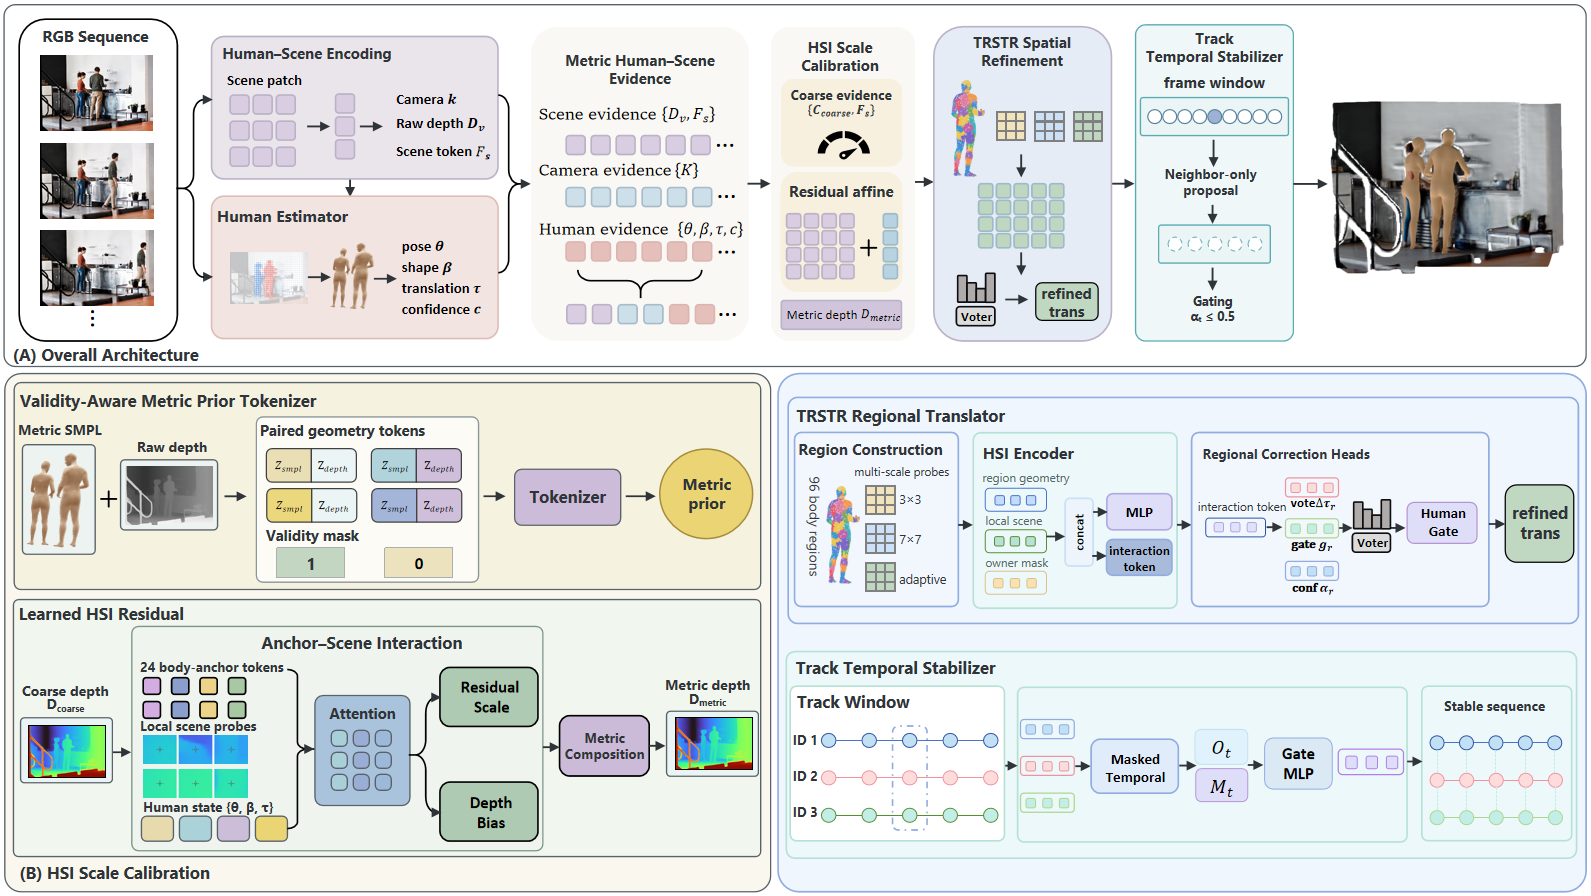
\includegraphics[width=\textwidth]{figures/main_method.png}
\caption{Overview of GroundedHuman. The input RGB sequence is processed by a scene encoder and a human observer, producing a metric human--scene evidence set consisting of a relative scene, camera, humans, and local geometry probes. HSI scale calibration first recovers a coarse scale from the human front surface and then predicts metric depth through a person-conditioned residual affine. TRSTR performs constrained spatial translation refinement over canonical human regions. Finally, a video-level trajectory stabilizer aggregates valid neighboring-frame evidence and shares the scale to output a scale-consistent 4D human--scene world.}
\label{fig:method-overview}
\end{figure*}

As shown in Fig.~\ref{fig:method-overview}, GroundedHuman organizes inference into the geometric chain ``observation--scale calibration--spatial refinement--trajectory stabilization.'' VGGT-Ω and NLF first extract scene and human observations from the same preprocessed images and form alignable metric human--scene evidence under a shared camera model. HSI scale calibration converts relative depth into metric depth; TRSTR then probes the scene around the human in the unified geometry and iteratively updates human translation. The video-level trajectory step does not introduce an independently claimed training module; it aggregates reliable-frame and neighboring-frame evidence at the clip level so that shared scale and camera translation remain in one temporal coordinate. Section 3.2 defines the observations and coordinate relation, Sec. 3.3 introduces analytic scale, Sec. 3.4 presents residual affine calibration, Sec. 3.5 describes regional translation refinement, and Sec. 3.6 gives the staged training objectives.

\subsection{Scene and Human Observations}

We use the scene reconstruction capability of VGGT-Ω as the relative geometric foundation without changing its original scene-inference path. For an input sequence, the VGGT-Ω aggregator updates image patch tokens, a camera token, and scene registers in a cross-frame context. The camera head outputs a 9D camera code from the camera token, including 3D translation, quaternion rotation, and horizontal and vertical fields of view; these quantities are decoded into camera-from-world extrinsics $\mathbf{T}_{cw,t}$ and full-image intrinsics $\mathbf{K}_t$. A dense prediction head recovers per-frame relative Z-depth $D_t^r$ from the aggregated patch features. We preserve the relative scene structure and camera rotation from VGGT-Ω and explicitly handle only the missing scale downstream.

Person-conditioned calibration also exposes multi-level scene representations from VGGT-Ω. We linearly project the patch features from the final four cached aggregator layers and concatenate them along the channel dimension to form a scene feature map queryable by human anchors. The multi-level representation places local appearance, depth boundaries, and cross-frame structural context in one feature space, allowing downstream modules to judge whether a correspondence is supported by surrounding scene evidence rather than relying on a single depth residual. All scene features remain frozen; new capacity is concentrated in the human-conditioned readout and geometric-refinement modules.

The human branch uses NLF as an external human observer. NLF receives the same resized and padded RGB tensor as VGGT-Ω rather than cropping into a separate image coordinate system. More importantly, we pass the $K_t$ decoded from the VGGT-Ω camera code into NLF, so human recovery, human projection, and scene-depth sampling share the same perspective camera. For every valid person slot, NLF outputs an SMPL axis-angle pose, 10D shape parameters, camera-space root translation, and confidence. We also convert the axis-angle pose into a continuous 6D rotation representation for subsequent HSI-token encoding.

Given the human parameters, the SMPL layer decodes vertices and joints in the local body coordinate system and adds the root translation to obtain a camera-space human. The $\texttt{i}$-th vertex is

\begin{equation}
\mathbf{X}_{tqi}^{h}
=\operatorname{SMPL}_{i}(\boldsymbol{\theta}_{tq},\boldsymbol{\beta}_{tq})
+\boldsymbol{\tau}_{tq}.
\label{eq:smpl-camera-vertices}
\end{equation}

In Eq.~(\plaineqref{eq:smpl-camera-vertices}), both $\mathbf{X}_{tqi}^{h}$ and $\boldsymbol{\tau}_{tq}$ are in meters and expressed in the camera coordinates of frame $t$. We consistently use the camera Z-depth convention; human anchors therefore use their Z component to establish a same-ray scale constraint with $D_t^r$. The same convention is used for analytic scale, depth back-projection, and TRSTR regional probing.

The two observations thus form a complementary geometric decomposition: VGGT-Ω provides a high-coverage relative scene, while NLF/SMPL provides a lower-coverage human surface with physical units. With both pretrained priors frozen, we explicitly establish their scale relation, decouple local human estimation, scene structure, and the new calibration modules, and allow scale recovery and translation refinement to be trained and validated independently.

\subsection{Human-anchored Analytic Coarse Scale}

We first decompose monocular scale recovery into analytic normalization and learned residual estimation. The former uses the metric Z-depth of the SMPL surface to remove the dominant scale gauge of the relative scene; the latter models only the unexplained residual after normalization. This decomposition converts large-range absolute-scale regression across scenes into local calibration around unit scale and provides downstream learning with an explicit, parameter-free geometric initialization that does not depend on test-time metric depth.

Concretely, we sparsely sample surface vertices from the SMPL mesh of each confident human at a fixed stride and use $\mathbf{K}_t$ to project camera-space vertices onto the VGGT-Ω depth plane. For a vertex $\mathbf{X}_{tqi}^{h}=(x_{tqi}^{h},y_{tqi}^{h},z_{tqi}^{h})$, its 2D projection $\mathbf{p}_{tqi}$ and scale candidate $a_{tqi}$ are

\begin{equation}
\mathbf{p}_{tqi}=\pi(\mathbf{K}_t,\mathbf{X}_{tqi}^{h}),\qquad
a_{tqi}=\frac{z_{tqi}^{h}}
{D_t^r\!\left(\left\lfloor\mathbf{p}_{tqi}\right\rceil\right)}.
\label{eq:analytic-anchor-ratio}
\end{equation}

Eq.~(\plaineqref{eq:analytic-anchor-ratio}) converts every visible human-surface point into an independent scale hypothesis. Unlike scale anchoring based on a single root joint or head depth, surface consensus produces an overconstrained estimate over the projected body region, so local joint errors or a single noisy depth sample cannot determine the global scale.

To make the scale hypotheses consistent with camera visibility, we apply a discrete z-buffer-like front-surface test to the projected human: for each pixel we retain only the human vertex with the smallest Z-depth, and discard out-of-image, non-positive-depth, invalid-scene-depth, and out-of-support correspondences. We denote this visibility-consistent anchor set by $\mathcal{A}_t$; its construction prevents an occluded surface from imposing a contradictory scale constraint on the same scene pixel.

We perform a robust location estimate over the scale hypotheses in $\mathcal{A}_t$ to obtain the frame-level analytic coarse scale:

\begin{equation}
s_t^c=\operatorname*{median}_{(q,i)\in\mathcal{A}_t}a_{tqi},
\qquad D_t^c=s_t^cD_t^r.
\label{eq:coarse-scale}
\end{equation}

Median aggregation suppresses the heavy-tailed ratios produced by depth boundaries and incorrect projections; estimating only a multiplicative scale restricts this stage to similarity-scale normalization. Valid surfaces from multiple people share the same $\mathcal{A}_t$ in a frame and therefore jointly constrain the scene scale rather than defining inconsistent local metric coordinates for each person.

For frames with severe truncation or insufficient support, we reject the low-confidence frame-level estimate and propagate a robust scale from the set of reliable frames \texttt{V} within the clip:

\begin{equation}
s_t^c\leftarrow
\exp\!\left(\operatorname*{median}_{u\in\mathcal{V}}\log s_u^c\right).
\label{eq:scale-fallback}
\end{equation}

This clip-level log-median is symmetric in multiplicative space and suppresses scale outliers in isolated frames. Its statistic is computed entirely from human--depth correspondences inside the video and introduces no test-set metric scale.

The analytic coarse scale is not intended to solve every depth error at once, but to reliably remove the dominant global ratio. Human initialization errors, local misalignment between the body and depth boundary, and additive bias in relative depth can still cause systematic differences between $D_t^c$ and the true metric depth. We therefore introduce a learned residual affine after coarse scaling in Sec. 3.4, allowing the network to focus on a narrower and more stable calibration range.

\subsection{Person-conditioned Residual Affine Calibration}

The analytic median uses only the Z-depth ratio between the human and scene at corresponding pixels, without explicitly judging the reliability of each local correspondence or representing residual bias in relative depth. We therefore design a person-conditioned residual-affine module that organizes SMPL parameters, local geometry probes, and VGGT-Ω scene features into a compact human--scene interaction representation. The module does not regenerate dense depth; it predicts only a residual scale $\rho_t$ and residual bias $b_t$ applied to the coarse depth $D_t^c$, preserving a clear division of responsibility between analytic scale and learned correction.

\subsubsection{Human--Scene Anchor Representation}

We construct 24 HSI anchor tokens for each person. This compact representation follows the idea in GRAFT of summarizing human--scene relations with a small set of body locations, adapted here for scale estimation. Twenty-one tokens correspond to non-root SMPL body joints; left and right hands each form one hand anchor by averaging adjacent wrist/hand joints; and a final global anchor is the mean of 27 fixed template vertices selected by deterministic farthest-point sampling. Joint anchors provide local geometric constraints at different limb locations, hand anchors cover extremities, and the global anchor encodes overall body location and shape.

Each anchor token contains both human state and human--scene relation. Human state consists of the 6D rotations of 24 joints, 10D shape parameters, and root translation, broadcast to every token; spatial state includes the anchor's camera coordinates and normalized 2D projection. For each anchor, we search a $9\times 9$ depth window around its projection for the valid scene point nearest in 3D distance, and compute the point location, human--scene 3D offset, Euclidean distance, scene normal, and Z-depth residual. If the local window has no valid candidate, we fall back to the depth at the projected anchor center. All attributes are projected by shared MLPs into 512D HSI tokens.

This tokenization explicitly factorizes the canonical human prior and observation residual: pose and shape determine the semantic identity and metric location of an anchor, while the local scene probe describes the deviation of current scene geometry from that anchor. Their joint encoding lets the residual heads compare scale evidence across body parts under shared human-coordinate semantics instead of implicitly compressing absolute-scale cues into one global image feature.

\subsubsection{Local Scene Attention}

Geometry probes and VGGT-Ω patch features provide explicit 3D residuals and cross-frame visual--geometric context, respectively. We project and concatenate the last four cached aggregator layers into a 512D scene representation, then extract a $3\times 3$ neighborhood of scene tokens around each anchor's 2D projection. This anchor-conditioned sparse connectivity constrains attention to a local bipartite graph with explicit projection correspondence, preserving multi-level scene evidence while suppressing information leakage from unrelated dynamic regions.

The HSI Transformer has five layers with shared structure. Each layer contains self-attention among human tokens, constrained cross-attention between an anchor and its local scene window, and a feed-forward network. Self-attention allows scale observations on different limbs to cross-check one another; for example, an occluded hand can receive context from stable torso and lower-limb observations. Cross-attention strictly restricts body token $\texttt{k}$ to scene tokens adjacent to its own projection, preserving an explicit 2D--3D correspondence. The hidden dimension is 512 with eight attention heads per layer; the five-layer Transformer is repeated three times in the current configuration to progressively integrate human-internal and local scene evidence.

\subsubsection{Multi-person Residual Affine}

After interaction, the 24 tokens are mean-pooled within each person to obtain a scene-calibration representation. Two independent MLP heads output the residual log-scale $\Delta\ell_{tq}$ and residual bias $\Delta b_{tq}$. Because visibility and detection reliability vary across people in a frame, we do not average person predictions directly; instead, we construct weights from nonnegative human confidence:

\begin{equation}
w_{tq}=
\frac{\max(c_{tq},0)}
{\max\!\left(\sum_j\max(c_{tj},0),\varepsilon\right)}.
\label{eq:person-confidence}
\end{equation}

Person predictions are first aggregated in log-scale space. The aggregated log-scale is clipped to the configured interval $[\ell_{\min},\ell_{\max}]$ and exponentiated to obtain a positive scale, while the bias is aggregated in linear space:

\begin{equation}
\ell_t=\operatorname{clip}\!\left(
\sum_q w_{tq}\Delta\ell_{tq},\ell_{\min},\ell_{\max}\right),
\quad \rho_t=\exp(\ell_t),
\quad b_t=\sum_qw_{tq}\Delta b_{tq}.
\label{eq:residual-affine}
\end{equation}

The frame-level metric depth is therefore

\begin{equation}
D_t^m=\rho_tD_t^c+b_t=(s_t^c\rho_t)D_t^r+b_t.
\label{eq:metric-depth}
\end{equation}

Log-domain aggregation acts directly on the multiplicative scale gauge, and the bounded mapping suppresses extreme predictions from a single person. When no valid person is available, aggregation keeps the identity residual $\rho_t=1,b_t=0$, so the learned module cannot arbitrarily alter the analytic result in the absence of human evidence.

\subsubsection{Video-level Scale Consistency and Trajectory Stabilization}

Frame-level residual affine is suitable for single-frame depth, but world reconstruction cannot allow adjacent frames to have independent arbitrary scales: a static scene would expand or contract over time and camera translations would not form a coherent trajectory. The Track Temporal Stabilizer in Fig.~\ref{fig:method-overview} is our video-level evidence-organization step. It does not replace VGGT-Ω or NLF and is not an additionally claimed separately trained network; it robustly aggregates valid human frames, neighboring-frame scale candidates, and camera-motion evidence. For world-space tasks, we first combine analytic coarse and residual scales and then use a shared affine over the full video:

\begin{equation}
\widetilde{s}_t=s_t^c\rho_t,\qquad
s^{\mathrm{clip}}=\exp\!\left(
\operatorname*{median}_t\log\widetilde{s}_t\right),\qquad
b^{\mathrm{clip}}=\operatorname*{median}_tb_t.
\label{eq:clip-affine}
\end{equation}

Equation~(\plaineqref{eq:clip-affine}) establishes a clip-level gauge on the combined effective scale rather than smoothing the analytic and residual terms separately. This preserves their coupling and suppresses scale jumps caused by anomalous human observations in individual frames; neighboring-frame validity checks and trajectory-level aggregation prevent short occlusions from directly propagating a frame outlier to the world trajectory. The final depth and camera extrinsics are

\begin{equation}
D_t^m=s^{\mathrm{clip}}D_t^r+b^{\mathrm{clip}},\qquad
\mathbf{T}_{cw,t}^{m}=
\left[\mathbf{R}_{cw,t}\mid s^{\mathrm{clip}}\mathbf{t}_{cw,t}\right].
\label{eq:camera-scale}
\end{equation}

To preserve projection geometry, only the similarity component $s^{\mathrm{clip}}$ acts on camera translation; the affine bias $b^{\mathrm{clip}}$ is restricted to the depth domain and camera rotation remains unchanged. Relative camera trajectories and the depth field consequently share one metric gauge, providing a consistent basis for transforming camera-space humans into world coordinates.

\subsection{Regional Translation Refinement}

After scene-scale calibration, the remaining error is mainly a displacement of the human root along the camera ray and tangent directions, which directly propagates to world-space joint error and root trajectory. We therefore restrict refinement to a translation-only subspace: TRSTR extracts scene-consistency evidence from multiple human-surface regions and aggregates it into one root-translation increment; $\theta$ and $\beta$ are treated as local-human invariants and remain fixed throughout refinement. The complete architecture of the human-scale bridge and TRSTR is moved to Appendix Fig.~\ref{fig:method-detail}.

\subsubsection{Deterministic Human Regions}

TRSTR uses an anatomical surface basis consistent with SMPL kinematics as its local interaction carrier. Each template vertex is first assigned to head/neck, torso, pelvis, upper limbs, hands, lower limbs, or feet according to its dominant LBS joint; deterministic farthest-point sampling is then performed within each anatomical domain, producing 96 nonuniform surface regions. Unlike image-dependent dynamic clustering, this partition is constructed once on the canonical template and propagated through SMPL deformation to any identity and pose, providing stable anatomical correspondence for region representations shared across frames and people.

For each region, the centroid of its deformed member vertices defines the interaction center, while eight fixed member vertices provide sparse surface support. The centroid determines the region projection and camera-ray basis; the representative set encodes its projected extent and 3D spread under the current pose. Region identity remains fixed while geometric state follows body deformation, giving TRSTR both canonical semantics and pose-dependent local surface geometry.

This canonical--deformed dual representation keeps region tokens stable across identities and mesh vertex densities while remaining geometrically sensitive to pose, scale, and current translation. Region reliability can therefore be learned under shared anatomical semantics, while probe locations update with the human state at every iteration without predefined contact labels or static 2D crops.

\subsubsection{Multi-scale Human--Scene Probing}

TRSTR constructs multi-support-domain geometric probes for every region. Region centroids and representative points are projected into the metric depth map; the maximum projected extent of representative points relative to the centroid determines an adaptive radius. We then collect four support domains in parallel: fixed $3\times 3$, fixed $7\times 7$, an adaptive region, and an outer annulus. These domains capture center correspondence, local tolerance, pose-dependent coverage, and outside-region environment, so local evidence retains comparable spatial semantics under projection-scale changes and initialization offsets.

Local depth in a multi-person scene is not a binary human/environment observation. We rasterize all valid SMPL surfaces into an instance-owned depth buffer and decompose every sample into self-surface, other-human, and environment categories. Self-surface and environment form separate probe channels; other-human does not enter environmental aggregation and contributes only an interference ratio to the region state. This instance-aware decomposition prevents a neighboring person from being interpreted as the support or collision surface of the current human, preserving person-specific interaction under crowding and mutual occlusion.

Each sample is encoded by its 3D displacement from the region centroid, Z-depth residual, normalized pixel displacement, radial position, residual between the representative surface and instance depth buffer, and category flag. A point encoder and masked-attention pooling then aggregate point states within every ``support domain $\times$ evidence channel'' pair, producing eight probe tokens and their valid-support ratios. The representation retains residual direction, scale, and source, allowing subsequent regional reasoning to distinguish geometric inconsistency from simple observation missingness.

Region centroid, surface extent, 2D projection, probe tokens, support ratios, other-human fraction, adaptive radius, and a 32D anatomical-group embedding jointly define the region state and are mapped to a 256D hidden representation. TRSTR thus jointly models human--scene residuals, local visibility, and instance interference on a fixed number of region tokens rather than compressing dense depth crops into opaque features with no provenance.

\subsubsection{Ray-constrained Regional Voting}

TRSTR models human translation as a camera-induced anisotropic error rather than homogeneous regression in global XYZ. For the center of region $r$ at iteration $k$, we construct a unit camera ray $\mathbf{e}_{\parallel}$ and orthogonal tangent-plane bases $\mathbf{e}_{x},\mathbf{e}_{y}$, and predict three bounded coefficients in this view-covariant basis:

\begin{equation}
\mathbf{v}_{tqr}^{(k)}
=\delta_{\parallel,tqr}^{(k)}\mathbf{e}_{\parallel,tqr}^{(k)}
+\delta_{x,tqr}^{(k)}\mathbf{e}_{x,tqr}^{(k)}
+\delta_{y,tqr}^{(k)}\mathbf{e}_{y,tqr}^{(k)},
\label{eq:regional-vote}
\end{equation}
\noindent where
$\lvert\delta_{\parallel}\rvert\le d_{\parallel}$,
$\lvert\delta_x\rvert,\lvert\delta_y\rvert\le d_{\perp}$.

$\mathbf{v}_{tqr}^{(k)}$ is the regional candidate vote for shared human translation, while $d_{\parallel}$ and $d_{\perp}$ define the depth and tangential trust regions. This parameterization binds network output to imaging geometry, keeps update directions semantically consistent across camera views, and allows different prior ranges for depth and lateral errors.

\subsubsection{Uncertainty-weighted Human Update}

Local probes are strongly heteroscedastic under occlusion, image boundaries, and missing depth. TRSTR therefore jointly predicts a candidate vote, region gate $g_{tqr}^{(k)}$, and log-variance $\ell_{tqr}^{(k)}$ for each region. Let $m_{tqr}^{(k)}$ be the observation mask determined jointly by valid support, person validity, and positive depth. The regional precision weight is

\begin{equation}
\alpha_{tqr}^{(k)}
=m_{tqr}^{(k)}g_{tqr}^{(k)}
\exp\!\left(-\ell_{tqr}^{(k)}\right).
\label{eq:precision-weight}
\end{equation}

Valid regions are weighted jointly by a learned gate and inverse variance, yielding a robust aggregation adaptive to local evidence quality:

\begin{equation}
\widehat{\mathbf{v}}_{tq}^{(k)}
=\frac{\sum_r\alpha_{tqr}^{(k)}\mathbf{v}_{tqr}^{(k)}}
{\max\!\left(\sum_r\alpha_{tqr}^{(k)},\varepsilon\right)}.
\label{eq:vote-aggregation}
\end{equation}

After regional aggregation, the module obtains a person-level representation from all valid region states and predicts a person gate. The final update is first component-wise clipped in camera XYZ coordinates and then multiplied by the person gate:

\begin{align}
\Delta\boldsymbol{\tau}_{tq}^{(k)}
&=g_{tq}^{\mathrm{person},(k)}
\operatorname{clip}_{\mathrm{component}}\!\left(
\widehat{\mathbf{v}}_{tq}^{(k)},-d_{\max},d_{\max}\right),
\label{eq:person-update}\\
\boldsymbol{\tau}_{tq}^{(k+1)}
&=\boldsymbol{\tau}_{tq}^{(k)}
+\Delta\boldsymbol{\tau}_{tq}^{(k)}.
\label{eq:translation-iteration}
\end{align}

$\operatorname{clip}_{\mathrm{component}}$ restricts the person-level update to a predefined trust region; together with the regional ray/tangent bounds, it forms a hierarchically bounded update. Combined with the region gate, heteroscedastic weights, and person gate, this mechanism prevents local outliers from being amplified without bound into a full-body displacement.

TRSTR uses shared weights for two geometric-loop iterations. After each update of $\boldsymbol{\tau}_{tq}$, the module redecodes the human surface with fixed $\boldsymbol{\theta}_{tq},\boldsymbol{\beta}_{tq}$, updates the region geometry, and recollects scene probes at the new projected locations. The second iteration therefore observes the residual distribution after the first transformation rather than repeatedly regressing the same static feature. The current model enables only this spatial loop and introduces no temporal state.

\subsection{Staged Training Objectives}

Scene-scale calibration and human translation refinement have different output spaces and error distributions, so we train them in stages rather than end-to-end optimizing the entire system. The scale module learns global affine parameters and must cover large scale variation in relative depth; TRSTR learns metric 3D translation and must handle correct initialization, small deviations, and severe misalignment. Staged training gives each module supervision consistent with its inference role and allows VGGT-Ω, NLF, and trained upstream components to remain frozen in later stages.

\subsubsection{Residual Scale Training}

The scale module is first pretrained on metric BEDLAM depth and GT SMPL using residual-gauge perturbations. We apply a shared log-normal perturbation to the full GT depth, randomizing the global scale gauge while preserving intra-sequence structure, and use the inverse perturbation as supervision. Training updates only the residual-scale and bias heads; VGGT-Ω, camera/depth heads, the HSI backbone, and human parameters remain frozen so the new heads specifically learn to recover the scale gauge from human--scene correspondences.

We then fine-tune the scale heads with coarse-residual stratified states that more closely match the real inference chain. Training first samples large-range absolute-scale perturbations of GT depth to create simulated scale-free depth, then estimates the coarse scale from the visible GT SMPL surface using the analytic algorithm in Sec. 3.3. To cover coarse-scale uncertainty caused by human initialization, projection, and local depth error, we further perturb the analytic result with four strata: identity, near, medium, and hard. The final residual target is the ratio between the absolute recovered scale and the coarse scale actually used, so the network predicts only the proportion unexplained by coarse normalization.

The scale teacher also comes from the visible human surface. After projecting GT SMPL vertices into the training depth, we select visible scene points consistent with human Z-depth in a local window and compute the ratio between human depth and input depth. Each human must have sufficient visible points, and frame-level scale candidates are robustly filtered by median absolute deviation. The median of the remaining candidates gives $\rho_t^*$. Current training uses no nonzero bias teacher; the bias is constrained by a zero target to prevent the model from abusing additive bias when a pure scale can explain the error.

The total scale-stage objective is

\begin{equation}
\mathcal{L}_{\mathrm{scale}}
=\lambda_s\mathcal{L}_{\log\text{-}\mathrm{scale}}
+\lambda_b\mathcal{L}_{\mathrm{bias}}
+\lambda_d\mathcal{L}_{\mathrm{depth}}.
\label{eq:scale-loss}
\end{equation}

Here $\mathcal{L}_{\log\text{-}\mathrm{scale}}$ is a Smooth-L1 loss between $\log\rho_t$ and $\log\rho_t^*$, $\mathcal{L}_{\mathrm{bias}}$ constrains the additive degree of freedom, and $\mathcal{L}_{\mathrm{depth}}$ supervises $\rho_tD_t^c+b_t$ on valid metric pixels. Joint supervision in parameter and geometric spaces constrains both the affine decomposition and final depth, avoiding equivalent but non-generalizable compensation between scale and bias.

\subsubsection{TRSTR Training}

After scale training, we freeze all upstream components and optimize only TRSTR region features, votes, region gates, log-variances, and the person gate. Training inputs are constructed from GT metric depth and GT SMPL, with states divided into clean, scale-error, NLF-like translation-error, and mixed-error. Scale-error applies a consistent small scale change to scene depth and target human position; NLF-like error injects root-translation noise of varying magnitude in the camera ray/tangent basis; mixed-error combines both. TRSTR consequently learns both to realign a human after scale changes and to correct depth and lateral offsets typical of an upstream human observer.

At each iteration, the supervision target does not require every region to output the full remaining displacement in one step. Instead, the residual from the current state to the target translation is divided by the number of remaining iterations to form a staged remaining-vote target. Only valid-region votes participate in regional supervision, while the region gate is trained with binary cross-entropy against the regional validity mask. The final person-level translation uses a Smooth-L1 loss against the target, constraining both local proposals and the aggregated full-body result.

The total TRSTR loss is

\begin{equation}
\begin{aligned}
\mathcal{L}_{\mathrm{TRSTR}}={}&
\lambda_{\mathrm{vote}}\mathcal{L}_{\mathrm{vote}}
+\lambda_{\mathrm{trans}}\mathcal{L}_{\mathrm{trans}}
+\lambda_{\mathrm{gate}}\mathcal{L}_{\mathrm{gate}}
+\lambda_{\mathrm{reg}}\mathcal{L}_{\mathrm{reg}}\\
&+\lambda_{\mathrm{strong}}\mathcal{L}_{\mathrm{strong}}
+\lambda_{\mathrm{id}}\mathcal{L}_{\mathrm{identity}}
+\lambda_{\mathrm{safe}}\mathcal{L}_{\mathrm{no\text{-}worse}}
+\lambda_{\mathrm{mono}}\mathcal{L}_{\mathrm{monotonic}}.
\end{aligned}
\label{eq:trstr-loss}
\end{equation}

Here $\mathcal{L}_{\mathrm{vote}}$ supervises staged translation proposals for valid regions, $\mathcal{L}_{\mathrm{trans}}$ supervises final human translation, $\mathcal{L}_{\mathrm{gate}}$ learns regional validity, and $\mathcal{L}_{\mathrm{reg}}$ constrains update magnitude. To preserve both large-error correction and local identity, we add four state-selective objectives: $\mathcal{L}_{\mathrm{strong}}$ strengthens recovery for states far from the target, $\mathcal{L}_{\mathrm{identity}}$ enforces a zero mapping for clean states, $\mathcal{L}_{\mathrm{no\text{-}worse}}$ penalizes degradation relative to initialization, and $\mathcal{L}_{\mathrm{monotonic}}$ constrains iterative error from increasing. These terms extend the objective from average regression to safe refinement sensitive to the initial error state.

Training defines scale and translation correction trajectories from GT geometry and controlled perturbations; inference uses only the VGGT-Ω relative scene, NLF human observations, and the calibration quantities predicted by our modules, without accessing GT depth, camera, or SMPL. The scale heads and TRSTR are optimized separately and executed sequentially, while VGGT-Ω and NLF remain frozen, yielding a modular scale-normalization and translation-refinement framework.

\section{Experiments}\label{sec:experiments}

We evaluate our method around three connected questions: whether local human pose and shape are preserved, whether the human-derived scale constraint improves world-space motion recovery, and whether it converts VGGT-Ω's scale-free depth into metric reconstruction consistent with both people and the environment. We evaluate local human meshes on 3DPW, global human motion on EMDB-2, and camera trajectories and human-centered video depth on TUM-Dynamic and Bonn, respectively. Together, these tasks validate the same human--scene reconstruction system from four perspectives: human quality, world trajectory, camera stability, and scene scale.

We use VGGT-Ω-1B-512 to predict scene depth and cameras, and NLF to provide human observations for human-related tasks. Unless otherwise stated, comparison values are taken from the public results of Human3R, UniSH, MetricHMSR, UniCon3R, and DuoMo; full training configurations and network hyperparameters are provided in the appendix.

To visualize the temporal output of GroundedHuman, Fig.~\ref{fig:temporal-4d} shows three representative video clips. Each row proceeds from input frames to the accumulated metric scene with time-coded human meshes in a shared world coordinate, followed by the human and camera world trajectories. The scene point cloud and human meshes in the middle use the same scale and coordinate gauge; the curves on the right show temporal trajectory continuity. This is a qualitative visualization and the curves are not an additional quantitative metric. The clips cover highly dynamic poses, outdoor walking/squatting, and sports scenes, testing whether human--scene relations remain coherent under viewpoint changes, local occlusion, and long sequences.

\begin{figure*}[t]
\centering
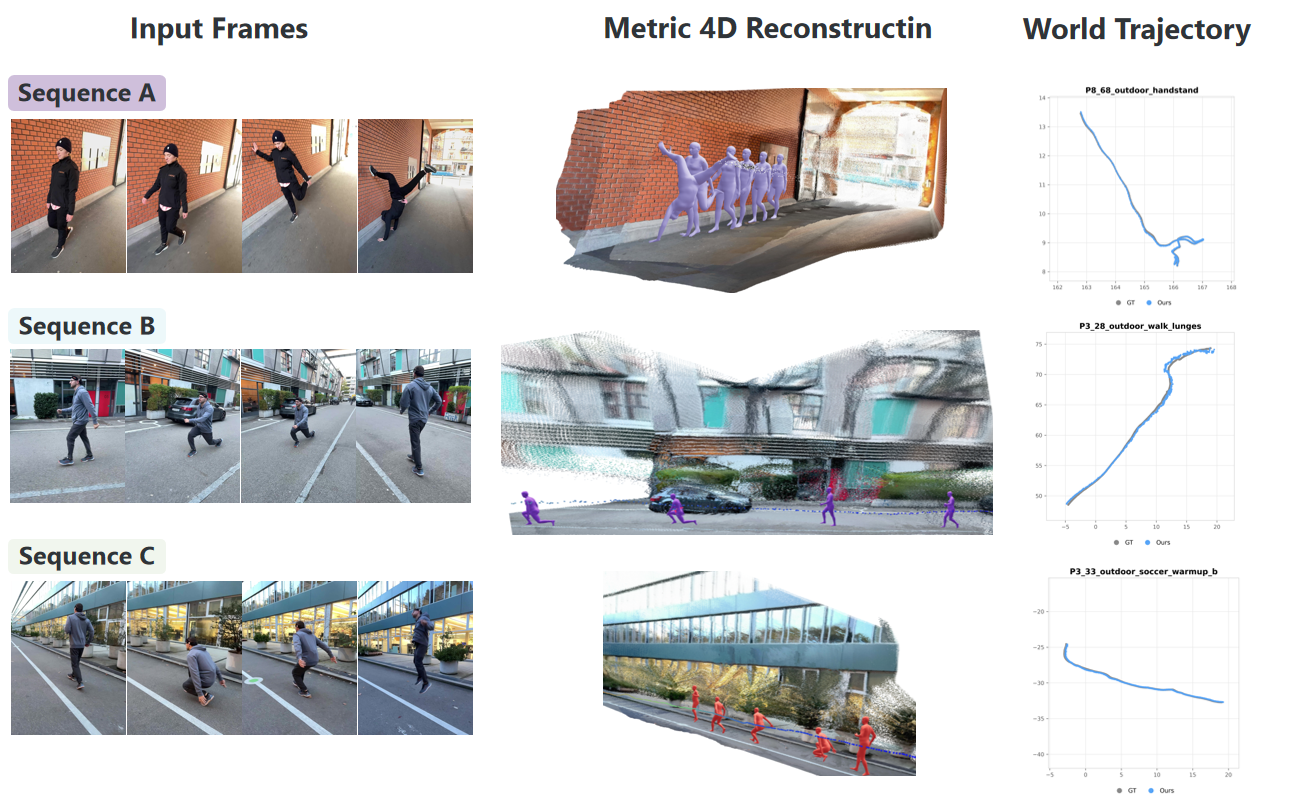
\includegraphics[width=\textwidth]{figures/fig3_temporal_4d.png}
\caption{Temporal human--scene reconstruction. Each row shows input video frames, an accumulated metric scene with time-coded human meshes, and human and camera trajectories in world coordinates from left to right. All frames are jointly visualized under the same scale and coordinate gauge; the curves on the right illustrate trajectory continuity and accuracy.}
\label{fig:temporal-4d}
\end{figure*}

\subsection{Local Human Mesh Recovery}

We first evaluate human pose and shape in camera coordinates on 3DPW. Following the Human3R protocol, we use PA-MPJPE, MPJPE, and PVE. PA-MPJPE measures pose structure after removing rigid transformation and scale; MPJPE and PVE measure joint and mesh-vertex error, respectively. We retain the EMDB-1 columns in Table~\ref{tab:local-hmr} to match the local-human evaluation format of Human3R.


\begin{table*}[t]
\caption{Local human mesh recovery on 3DPW and EMDB-1. ``\cmarkcolor'' indicates that the corresponding input is not required. All errors are in mm; lower is better.}
\label{tab:local-hmr}
\centering
\resizebox{\textwidth}{!}{%
\begin{tabular}{@{}lccc|ccc|ccc@{}}
\toprule
\multicolumn{1}{c}{Method} & \multicolumn{1}{c}{Crop-free} & \multicolumn{1}{c}{Detection-free} & \multicolumn{1}{c|}{Intrinsic-free} & \multicolumn{3}{c|}{3DPW (14)} & \multicolumn{3}{c}{EMDB-1 (24)} \\
\cmidrule(lr){5-7}\cmidrule(lr){8-10}
 & & & & PA-MPJPE $\downarrow$ & MPJPE $\downarrow$ & PVE $\downarrow$ & PA-MPJPE $\downarrow$ & MPJPE $\downarrow$ & PVE $\downarrow$ \\
\midrule
CLIFF & \xmarkcolor & \xmarkcolor & \xmarkcolor & 43.0 & 69.0 & 81.2 & 68.3 & 103.3 & 123.7 \\
HMR2.0 & \xmarkcolor & \xmarkcolor & \cmarkcolor & 44.4 & 69.8 & 82.2 & 61.5 & 97.8 & 120.0 \\
ReFit & \xmarkcolor & \xmarkcolor & \xmarkcolor & -- & -- & -- & 58.6 & 88.0 & 104.5 \\
TokenHMR & \xmarkcolor & \xmarkcolor & \cmarkcolor & 44.3 & 71.0 & 84.6 & 55.6 & 91.7 & 109.4 \\
CameraHMR & \xmarkcolor & \xmarkcolor & \cmarkcolor & 38.5 & 62.1 & 72.9 & 43.7 & 73.0 & 85.4 \\
BEV & \cmarkcolor & \cmarkcolor & \cmarkcolor & 46.9 & 78.5 & 92.3 & 70.9 & 112.2 & 133.4 \\
Multi-HMR & \cmarkcolor & \cmarkcolor & \xmarkcolor & 45.9 & 73.1 & 87.1 & 50.1 & 81.6 & 95.7 \\
Human3R & \cmarkcolor & \cmarkcolor & \cmarkcolor & 44.1 & 71.2 & 84.9 & 48.5 & 73.9 & 86.0 \\
\textbf{Ours} & \xmarkcolor & \xmarkcolor & \cmarkcolor & \textbf{37.3} & \textbf{60.3} & \textbf{71.4} & \textbf{--} & \textbf{--} & \textbf{--} \\
\bottomrule
\end{tabular}
}
\end{table*}

We obtain 37.3 mm PA-MPJPE, 60.3 mm MPJPE, and 71.4 mm PVE. Because the system directly preserves the pose and shape produced by the frozen human observer, while scale calibration and TRSTR only process scene scale and human root translation, these results verify that global geometric correction does not damage the local human mesh.

Compared with Human3R, our PA-MPJPE, MPJPE, and PVE are lower by 15.4\%, 15.3\%, and 15.9\%, respectively. Using a reliable human pose as the metric anchor allows the learned capacity to focus on scene scale and global-position calibration while fully preserving local human quality and providing a stable body-scale reference for subsequent world-space reconstruction.

\subsection{Global Human Motion in World Coordinates}

We evaluate world-space human motion and root trajectories on EMDB-2. Following Human3R and UniSH, long sequences are split into clips of at most 100 frames. WA-MPJPE estimates an alignment transform over the full clip and reflects overall motion accuracy; W-MPJPE aligns only the first two frames and is more sensitive to subsequent scale drift and accumulated trajectory error; RTE measures root-trajectory error after rigid alignment. Table~\ref{tab:global-motion} also reports RICH results to distinguish performance under dynamic cameras and different scene conditions.


\begin{table*}[t]
\caption{Global human motion estimation on EMDB-2 and RICH. In the preprocessed-input columns, ``\cmarkcolor'' indicates that the corresponding external input is not required; in the output columns, ``\cmarkcolor'' indicates that the method supports the capability and ``\xmarkcolor'' indicates that it is unsupported or not produced as a model output. Joint errors are in mm and RTE is in \%; lower is better for all metrics.}
\label{tab:global-motion}
\centering
\resizebox{\textwidth}{!}{%
\begin{tabular}{@{}llcccc|ccc|ccc|ccc@{}}
\toprule
\multirow{2}{*}{Category} & \multirow{2}{*}{Method} & \multicolumn{4}{c|}{Preprocessed Input ($\cmarkcolor$ = not required)} & \multicolumn{3}{c|}{Output} & \multicolumn{3}{c|}{EMDB-2 (24)} & \multicolumn{3}{c}{RICH (24)} \\
\cmidrule(lr){3-6}\cmidrule(lr){7-9}\cmidrule(lr){10-12}\cmidrule(lr){13-15}
 & & Tracking & Camera & Depth & Contact & Multi-Person & Metric Human--Scene & Contact-Aware & WA-MPJPE $\downarrow$ & W-MPJPE $\downarrow$ & RTE $\downarrow$ & WA-MPJPE $\downarrow$ & W-MPJPE $\downarrow$ & RTE $\downarrow$ \\
\midrule
\multirow{7}{*}{Offline} & GLAMR & \xmarkcolor & \cmarkcolor & \cmarkcolor & \cmarkcolor & \cmarkcolor & \xmarkcolor & \xmarkcolor & 280.8 & 726.6 & 11.4 & 129.4 & 236.2 & 3.8 \\
 & SLAHMR & \xmarkcolor & \xmarkcolor & \cmarkcolor & \cmarkcolor & \cmarkcolor & \xmarkcolor & \xmarkcolor & 326.9 & 776.1 & 10.2 & 132.2 & 237.1 & 6.4 \\
 & COIN & \xmarkcolor & \xmarkcolor & \cmarkcolor & \cmarkcolor & \xmarkcolor & \xmarkcolor & \xmarkcolor & 152.8 & 407.3 & 3.5 & 169.5 & 254.5 & -- \\
 & GVHMR & \xmarkcolor & \xmarkcolor & \cmarkcolor & \cmarkcolor & \xmarkcolor & \xmarkcolor & \xmarkcolor & 111.0 & 276.5 & 2.0 & 78.8 & 126.3 & 2.4 \\
 & TRAM & \xmarkcolor & \xmarkcolor & \xmarkcolor & \cmarkcolor & \xmarkcolor & \xmarkcolor & \xmarkcolor & 76.4 & 222.4 & 1.4 & 127.8 & 238.0 & 6.0 \\
 & JOSH & \xmarkcolor & \xmarkcolor & \xmarkcolor & \xmarkcolor & \cmarkcolor & \cmarkcolor & \cmarkcolor & 68.9 & 174.7 & 1.3 & 89.0 & 132.5 & 3.0 \\
 & PromptHMR & \cmarkcolor & \cmarkcolor & \cmarkcolor & \cmarkcolor & \xmarkcolor & \xmarkcolor & \xmarkcolor & 71.0 & 216.5 & 1.3 & 118.2 & 207.0 & 5.6 \\
\midrule
\multirow{8}{*}{Online} & TRACE & \cmarkcolor & \cmarkcolor & \cmarkcolor & \cmarkcolor & \cmarkcolor & \xmarkcolor & \xmarkcolor & 529.0 & 1702.3 & 17.7 & 238.1 & 925.4 & 610.4 \\
 & WHAM & \xmarkcolor & \xmarkcolor & \cmarkcolor & \cmarkcolor & \xmarkcolor & \xmarkcolor & \xmarkcolor & 135.6 & 354.8 & 6.0 & 108.4 & 196.1 & 4.5 \\
 & JOSH3R & \xmarkcolor & \xmarkcolor & \xmarkcolor & \xmarkcolor & \xmarkcolor & \cmarkcolor & \xmarkcolor & 220.0 & 661.7 & 13.1 & -- & -- & -- \\
 & Human3R & \cmarkcolor & \cmarkcolor & \cmarkcolor & \cmarkcolor & \cmarkcolor & \cmarkcolor & \xmarkcolor & 112.2 & 267.9 & 2.2 & 110.0 & 184.9 & 3.3 \\
 & MetricHMSR & \xmarkcolor & \xmarkcolor & \xmarkcolor & \xmarkcolor & \xmarkcolor & \cmarkcolor & \xmarkcolor & 72.1 & 199.5 & 1.4 & 109.6 & 165.5 & 1.9 \\
 & UniCon3R & \xmarkcolor & \xmarkcolor & \xmarkcolor & \xmarkcolor & \xmarkcolor & \cmarkcolor & \cmarkcolor & 113.7 & 285.6 & 2.3 & 81.5 & 129.8 & 1.7 \\
 & UniSH & \xmarkcolor & \xmarkcolor & \xmarkcolor & \xmarkcolor & \xmarkcolor & \cmarkcolor & \xmarkcolor & 118.5 & 270.1 & 5.8 & 118.1 & 183.2 & 4.8 \\
 & \textbf{Ours} & \cmarkcolor & \cmarkcolor & \cmarkcolor & \cmarkcolor & \cmarkcolor & \cmarkcolor & \cmarkcolor & \textbf{58.468} & \textbf{149.959} & \textbf{1.079} & -- & -- & -- \\
\bottomrule
\end{tabular}
}
\end{table*}

On EMDB-2, we obtain 58.468 mm WA-MPJPE, 149.959 mm W-MPJPE, and 1.079\% RTE. Relative to JOSH, the three errors decrease by 15.1\%, 14.2\%, and 17.0\%; relative to Human3R, by 47.9\%, 44.0\%, and 51.0\%; and relative to UniSH, by 50.7\%, 44.5\%, and 81.4\%, respectively.

The W-MPJPE improvement is more diagnostic of our method than a change in local human metrics. Because W-MPJPE aligns only at the start of a clip, subsequent error directly exposes accumulated scale and camera-motion bias. While preserving the NLF local-human result, we reduce W-MPJPE to 149.959 mm, indicating that the human-scale anchor primarily corrects the camera-to-world geometry. The lower WA-MPJPE and RTE further show that the benefit appears in both within-clip motion structure and the complete root trajectory.

\textbf{Human--scene interaction.} World-space trajectory metrics measure global motion accuracy, but do not fully capture the local geometric relationship between a human and the nearby environment. Following the qualitative comparison protocol of GRAFT~\citep{ym2026graft}, Fig.~\ref{fig:human-scene-interaction} compares UniSH, Human3R, and our method in lying, leaning, sitting, and two-person scenes. Existing methods can place people in the reconstructed scene, but floating, penetration, or front--back depth offsets remain visible near support surfaces. Our method places the human and environment in a shared metric coordinate system and uses TRSTR's local geometric evidence to refine root translation, producing support relationships between the torso, limbs, seats, and ground that better agree with the input observations. In the indoor sofa and outdoor bench examples, this improvement does not rely on pose or shape updates, indicating that constrained translation refinement directly improves geometric human placement.

\begin{figure*}[t]
\centering
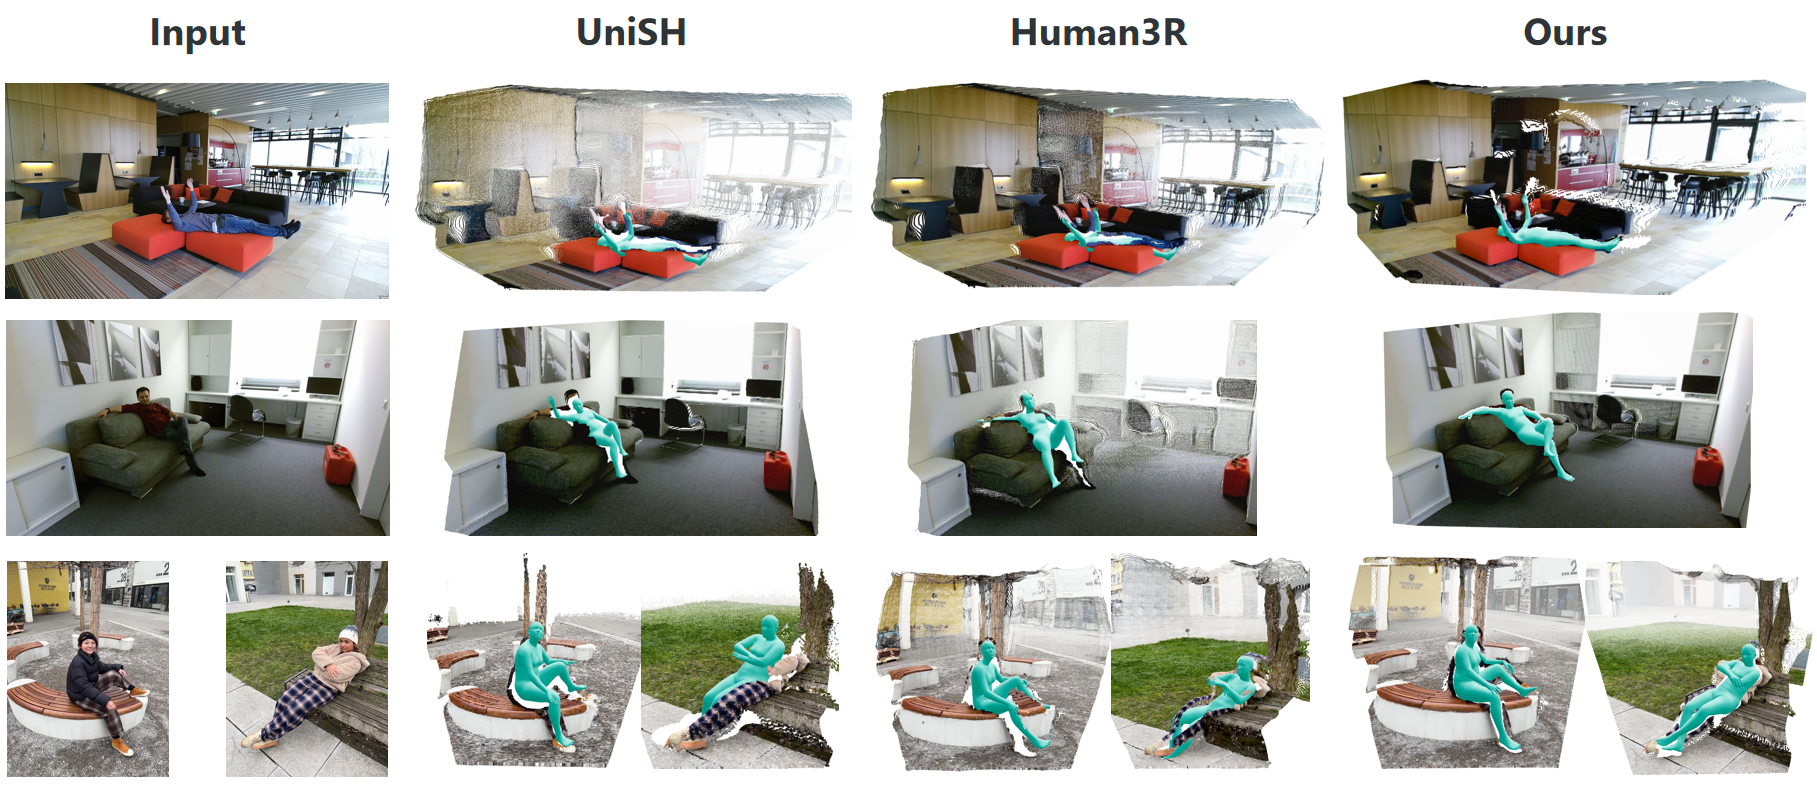
\includegraphics[width=\textwidth]{figures/fig_human_scene_interaction.png}
\caption{\textbf{Qualitative comparison of human--scene geometric interaction.} Each row shows the input image, UniSH, Human3R, and our joint human--scene reconstruction from left to right. Compared with the floating, penetration, and depth misalignment visible in the baselines, our method obtains root positions that better conform to scene surfaces and more coherent support relationships while preserving local human pose and shape. This figure provides qualitative evidence of geometric interaction; global motion and metric-scene performance are evaluated quantitatively in Table~\ref{tab:global-motion} and Appendix Table~\ref{tab:bonn-depth}, respectively.}
\label{fig:human-scene-interaction}
\end{figure*}

\subsection{General 3D Reconstruction}

\textbf{Camera pose estimation.} We first evaluate camera trajectories on TUM-Dynamic. Following Human3R, we align the predicted trajectory with Sim(3) and compute absolute trajectory error (ATE). As shown in Fig.~\ref{fig:general-reconstruction}(a), the ATE of VGGT-Ω at 50, 100, 150, 200, 300, 400, and 500 input views is 0.00299, 0.00434, 0.00493, 0.00591, 0.00634, 0.00645, and 0.00692 m, respectively. Even as input length grows from 50 to 500, the increase remains below 4 mm and all evaluation points stay below 7 mm. In contrast, the Human3R reference curve grows from approximately 0.013 m to 0.052 m. At 500 views, VGGT-Ω reduces ATE by about 86.7\%, indicating little trajectory drift as the sequence length increases.

\begin{figure*}[t]
\centering
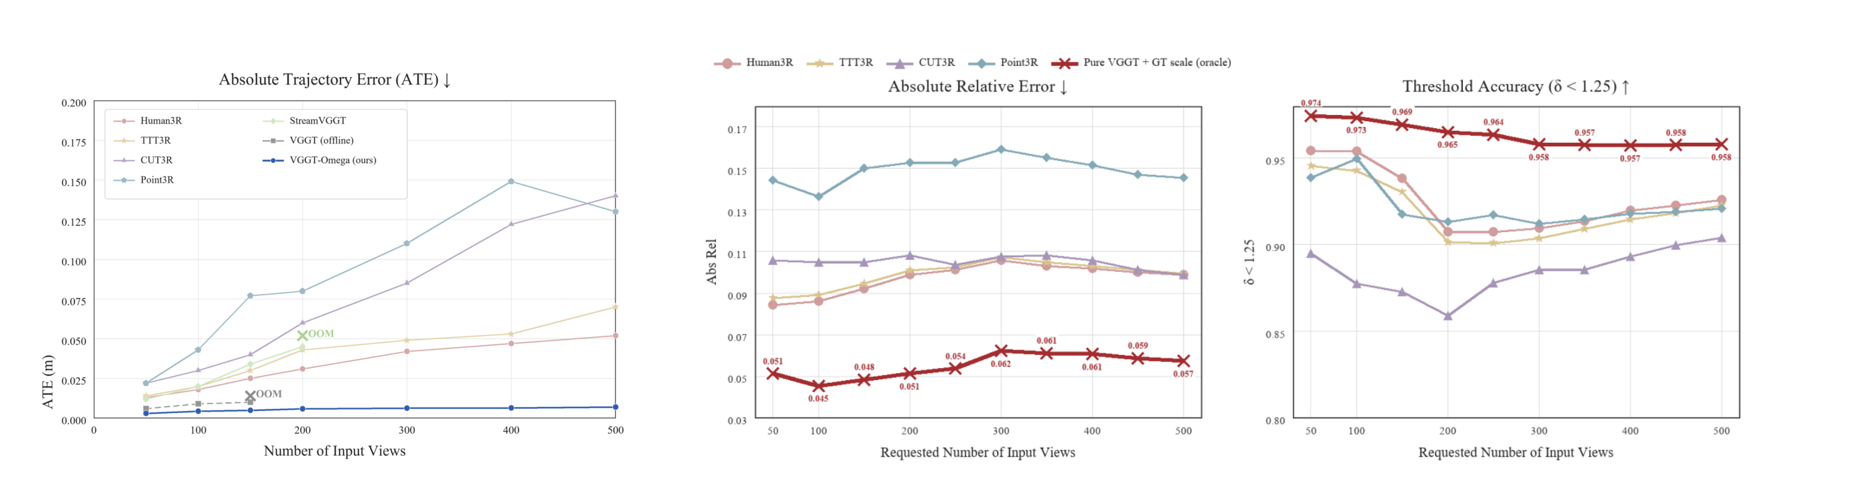
\includegraphics[width=\textwidth]{figures/fig_generic_3d_reconstruction_curves.png}
\caption{\textbf{General 3D reconstruction evaluation.} (a) Camera-trajectory ATE on TUM-Dynamic as the number of input views changes; (b-c) Abs Rel and $\delta<1.25$ on Bonn as the requested number of input views changes. The blue VGGT-Ω ATE curve is obtained from our exact evaluator; the camera and depth reference curves are approximately digitized from Fig. 9 of Human3R. The red Bonn curves are an oracle diagnostic for Pure VGGT + GT scale: each sequence and input prefix uses a scale fitted from GT, only to analyze a measurable upper bound of VGGT-Ω relative geometry, not as a privileged prediction of our method. The x-axis is the requested maximum number of views; shorter sequences use all available frames without repeated padding.}
\label{fig:general-reconstruction}
\end{figure*}

\textbf{Video depth estimation.} We next evaluate human-centered video depth on Bonn. The complete comparison is reported in Appendix Table~\ref{tab:bonn-depth}. Our results are computed directly from the human-scale-calibrated model output using Abs Rel and $\delta<1.25$, without GT scale or shift at evaluation time. This setting measures not only relative scene structure, but also cross-frame scale and absolute-depth consistency.

We obtain 0.08599 Abs Rel and 0.96377 $\delta<1.25$ accuracy. Compared with Human3R, we maintain a comparable Abs Rel while improving threshold accuracy by 0.98 percentage points; compared with CUT3R, $\delta<1.25$ improves by 2.68 points; and the gap to VGGT is only 0.22 points. Importantly, these results are obtained directly from VGGT-Ω depth calibrated by the human metric anchor, without GT scale or shift during evaluation. The result shows that even when the scene model does not provide reliable absolute scale, human physical size can calibrate most scene pixels into the 1.25-times-correct-depth range.

Fig.~\ref{fig:general-reconstruction}(b-c) further provides an oracle-scale diagnostic for VGGT-Ω relative depth. Over 50 to 500 requested views, fitting one GT scale gives Abs Rel between 0.045 and 0.062 and $\delta<1.25$ between 0.957 and 0.974; at 500 views it still reaches 0.057 Abs Rel and 0.958 threshold accuracy. This indicates that VGGT-Ω already recovers stable relative scene structure and identifies absolute-scale recognition as a key bottleneck. We replace the oracle scale source with human physical size and obtain 0.96377 threshold accuracy, verifying that a human can provide an effective metric reference for scale-free scene geometry.

\clearpage
\begin{wrapfigure}[27]{r}{0.48\textwidth}
\vspace{-0.5\baselineskip}
\centering
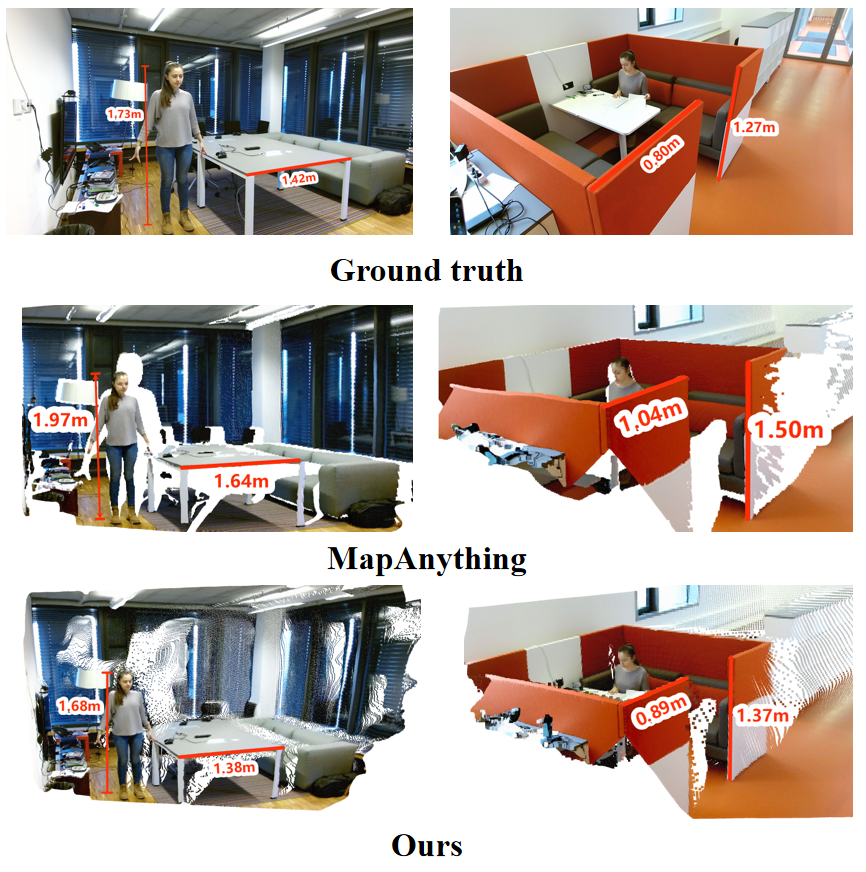
\includegraphics[width=0.46\textwidth]{figures/fig_metric_measurement.png}
\caption{\textbf{Qualitative comparison of real-world measurements.} The two columns show different indoor scenes; the three rows show Ground Truth, MapAnything, and our method. Red annotations denote human heights or object lengths measured from reconstructed geometry; quantitative results are given in Appendix Table~\ref{tab:bonn-depth}.}
\label{fig:metric-measurement}
\end{wrapfigure}

Fig.~\ref{fig:metric-measurement} complements the pixel-level evaluation above from the perspective of object scale. For each scene, Ground Truth, MapAnything, and our method expose the length relationship between the human and environment geometry. GroundedHuman produces a human height and several environmental measurements closer to reality, while keeping the human and reference objects such as tables and partitions in the same metric range. This agrees with the Bonn depth result without GT scale or shift: human anchoring provides pixel-level depth calibration and makes the reconstruction interpretable as scene geometry with real-world length. Because occlusion and local depth noise still affect individual objects, we present this figure qualitatively and do not extrapolate a single-object error into a new benchmark metric.

\subsection{Scale-consistency Analysis}

The three experiments form a consistent chain of evidence. First, the local-human errors on 3DPW, identical to NLF, show that scale calibration does not improve global metrics by changing human pose or shape. Second, the leading WA-MPJPE, W-MPJPE, and RTE on EMDB-2 show improvements in world-space motion structure, long-term drift, and root trajectories. Finally, the long-sequence ATE below 7 mm on TUM-Dynamic independently indicates that the scene backbone has a stable camera trajectory; the Bonn oracle diagnostic further identifies absolute-scale recognition as a key bottleneck, while our 0.96377 threshold accuracy demonstrates that the scale can be supplied by a human.

Together, these results validate our core design: the human first provides a global scale anchor, and local human--scene evidence then refines human translation. The former establishes a metric scale shared by people and environment; the latter reduces local human misplacement in the scene. GroundedHuman consequently improves world trajectories, stabilizes camera motion, and yields scale-consistent scene depth while preserving local human quality.

\section{Conclusion}\label{sec:conclusion}

We studied scale-consistent reconstruction of scenes, cameras, and humans from monocular video and validated a central idea: even when a scene foundation model provides only stable relative geometry, a parametric human with metric meaning can serve as an intrinsic metric reference in the video. We first remove the dominant scene-scale gauge through scale consensus over the visible SMPL front surface, then use a person-conditioned residual affine to correct residual scale and depth bias and propagate a shared clip-level scale to camera translation. TRSTR subsequently uses canonical anatomical regions as local geometric probes and gated, uncertainty-weighted iterative votes to correct only human root translation while preserving pose and shape. The 3DPW result shows that local human accuracy is preserved; 58.468 mm WA-MPJPE, 149.959 mm W-MPJPE, and 1.079\% RTE on EMDB-2 validate scale-consistent world motion and root trajectories; and 0.08599 Abs Rel and 0.96377 $\delta<1.25$ without GT scale/shift on Bonn show that a human can turn a relative scene into effective metric depth. Together with the stable long-sequence camera trajectory on TUM-Dynamic, these results form a consistent evidence chain from local humans and scene scale to world motion.

The applicability of our method still depends on the quality of upstream scene and human observations. When a person is invisible for a long period, severely truncated, or absent from a clip, the human scale anchor weakens; incorrect relative scene structure or SMPL shape and translation also propagate into later calibration. TRSTR is intentionally restricted to a translation-only subspace and therefore cannot correct incorrect pose, shape, or fine-grained contact; the current implementation also uses only spatial regional evidence. Future work can introduce cross-frame scale-confidence aggregation, region memory under occlusion, and controlled human--scene contact constraints while preserving local HMR invariance, extending metric anchoring to longer, more crowded, and more interactive videos.

\subsubsection*{Acknowledgments}

Omitted in the double-blind review version.



\subsection*{Generative AI Use Disclosure}
Generative AI tools were used to assist with the organization and language editing of the Chinese draft, its English translation, and early sketches of conceptual figures.
All technical designs, code, experimental data, equations, literature claims, and final content were reviewed by the authors;
the authors take full responsibility for the contents of this paper.

\subsection*{Ethics Statement}
This work uses public human and scene research datasets for method development and evaluation, and does not target identity recognition or individual-attribute inference. Human-video reconstruction may raise privacy concerns, risks of surveillance misuse, and scale bias across body types; Appendix~\ref{app:limitations} discusses these boundaries. Dataset licenses and conditions of use will be checked individually before final submission, and no unverified information is inferred in this manuscript.

\subsection*{Reproducibility Statement}
The appendix documents coordinate and scale conventions, the complete inference procedure, training objectives, datasets, and evaluation protocols, and explicitly marks ablation, robustness, and efficiency results that still require real experiments. Before final submission, all placeholders will be replaced with verified server configurations, anonymous code, execution scripts, and real experimental outputs. No quantitative conclusion in this paper is supported by placeholder content.

\bibliography{references}
\bibliographystyle{iclr2027_conference}

\clearpage
\appendix
\section{Data Curation, Evaluation Protocols, and Complete Depth Results}
\label{app:bonn-results}

Following the organization of the UniSH supplementary material, we first state the data and filtering boundaries before presenting the complete evaluation. This work uses the public 3DPW, EMDB, TUM-Dynamic, and Bonn datasets for their corresponding tasks; v0.3 does not claim to construct a new training dataset or a new collection of web videos. The final version must report the exact splits, number of valid samples, crop and resize operations, human-visibility rules, invalid-depth masks, and dataset licenses. Any filtering threshold that has not yet been verified remains explicitly marked as pending.

Table~\ref{tab:bonn-depth} is the original Table 3 moved from the main paper to the appendix. Our result is computed from the human-scale-calibrated model output without using GT scale or shift at test time. The red curves in Fig.~\ref{fig:general-reconstruction}, which fit a scale from GT, are oracle diagnostics only and are not predictions of our method. The remaining appendices document coordinate conventions, model architecture, training configuration, component impact, robustness, efficiency, and failure analysis.

\begin{table}[H]
\caption{Human-centered video depth estimation on Bonn. Lower Abs Rel and higher $\delta<1.25$ are better.}
\label{tab:bonn-depth}
\centering
\begin{tabular}{lcc}
\toprule
Method & Abs Rel $\downarrow$ & $\delta<1.25$ $\uparrow$ \\
\midrule
DUSt3R & 0.151 & 0.839 \\
MASt3R & 0.188 & 0.765 \\
MonST3R & 0.072 & 0.957 \\
Fast3R & 0.194 & 0.772 \\
MVDUSt3R & 0.426 & 0.357 \\
CUT3R & 0.078 & 0.937 \\
Aether & 0.273 & 0.594 \\
FLARE & 0.152 & 0.790 \\
VGGT & 0.057 & 0.966 \\
$\pi^3$ & 0.049 & 0.975 \\
Human3R & 0.086 & 0.954 \\
UniSH & \textbf{0.035} & \textbf{0.980} \\
\textbf{Ours} & 0.08599 & 0.96377 \\
\bottomrule
\end{tabular}
\end{table}

\section{Notation, Coordinate Systems, and Metric Gauge}
\label{app:coordinates}

This appendix provides implementation and evaluation details omitted from the main paper for clarity. Appendix~\ref{app:coordinates} specifies coordinate and scale conventions; Appendix~\ref{app:architecture} gives the complete inference procedure; Appendix~\ref{app:training} summarizes the training objectives; Appendix~\ref{app:evaluation} describes datasets and evaluation protocols; Appendices~\ref{app:ablation}--\ref{app:efficiency} reserve the real ablation, robustness, and efficiency results; and Appendix~\ref{app:limitations} records failure modes and responsible-use boundaries. Every red ``To be evaluated'' entry is an explicit placeholder and does not constitute a result or supporting evidence.

\subsection{Coordinate and Depth Conventions}

For frame $t$ and person $n$ in a clip, VGGT-Ω predicts relative scene depth and camera parameters, while NLF provides SMPL human observations expressed in meters. We establish correspondences between human surfaces and scene depth using Z-depth along the camera optical axis; Euclidean distance along a camera ray is not treated as Z-depth. Camera coordinates, world coordinates, camera-to-world transformations, and matrix multiplication follow the conventions of Eqs.~\ref{eq:metric-depth-overview}--\ref{eq:translation-overview}.

Let $D^{\mathrm{rel}}$ denote relative depth, $s_{\mathrm{clip}}$ the shared clip-level scale, and $b_{\mathrm{clip}}$ the residual depth bias. Metric depth and metric camera translation are
\begin{equation}
D^{\mathrm{metric}} = s_{\mathrm{clip}}D^{\mathrm{rel}} + b_{\mathrm{clip}},
\qquad
\mathbf{t}^{\mathrm{metric}} = s_{\mathrm{clip}}\mathbf{t}^{\mathrm{rel}}.
\label{eq:appendix-metric-propagation}
\end{equation}
The bias acts only in the depth domain and is not directly added to camera translation. After shared-scale propagation, TRSTR performs a constrained camera-space translation update on the human root, while pose and shape remain frozen.

\subsection{Tensor, Precision, and Device Conventions}

\begin{table}[H]
\caption{Main tensors and implementation conventions. Exact dimensions follow the final implementation configuration.}
\label{tab:tensor-conventions}
\centering
\small
\begin{tabular}{llll}
\toprule
Object & Main dimensions & Unit/coordinates & Status \\
\midrule
Input images & $B\times T\times3\times H\times W$ & image plane & defined \\
Relative depth & $B\times T\times H\times W$ & relative Z-depth & defined \\
SMPL vertices & $B\times T\times N\times V\times3$ & camera, meter & defined \\
Human anchors & $B\times T\times N\times24\times C$ & feature space & defined \\
TRSTR regions & $B\times T\times N\times96\times C_r$ & canonical body & defined \\
Exact dtype/device & -- & -- & \todoresult \\
\bottomrule
\end{tabular}
\end{table}

\section{Model Architecture Details and Complete Inference}
\label{app:architecture}

\subsection{VGGT-Ω, NLF, and Baseline Boundaries}

VGGT-Ω provides relative scene structure, camera parameters, and multi-level scene features. NLF provides local human pose, shape, camera-space translation, and confidence. GroundedHuman does not replace either baseline, and TRSTR is not allowed to reduce world-space error by changing pose or shape. The final version must list frozen parameters, trainable parameters, input resolution, clip length, and the maximum number of person slots.

\placeholdernote{The frozen-module inventory, checkpoint paths, input shapes, dtypes, devices, and memory configuration must be verified against the server implementation.}

\subsection{Visible-front-surface Analytic Scale}

For every valid person, the SMPL surface is projected into the relative-depth map, and a z-buffer-like front-surface test retains the visible body surface closest to the camera at shared pixels. Ratios between human Z-depth and relative scene Z-depth at valid pixels form scale proposals; a robust median removes the dominant scale freedom. In multi-person scenes, person-level proposals are aggregated into a clip-scale candidate according to visible support and confidence.

The final version must report the minimum number of valid pixels, depth-boundary exclusion radius, MAD or outlier threshold, ratio clamp, $\varepsilon$, low-confidence fallback, and handling of clips without a visible person.

\subsection{Person-conditioned Residual Affine}

Each person is represented by 24 canonical anchors. The module queries local depth residuals and multi-level VGGT-Ω scene features near the projected human, and outputs a near-identity residual scale and depth bias. Analytic geometry determines the scale magnitude; the learned module models only residual errors caused by occlusion, projection, and local depth bias.

\placeholdernote{Transformer/MLP depth, hidden dimension, attention heads, normalization, initialization, output range, and anchor fallback must be filled from the verified configuration.}

\subsection{Clip-level Consensus and Camera Propagation}

Frame- and person-level scales are first aggregated over valid people and then combined into a shared clip scale, which acts on both scene depth and camera translation. Frames with short-term human invisibility should reuse or smooth a reliable clip scale. The fallback for long intervals without a person must be explicitly specified; the latest valid scale must not be propagated indefinitely by default.

\subsection{Complete TRSTR Update}

TRSTR organizes the SMPL surface into 96 canonical body regions and separately samples self-surface, environment, and other-human geometry around each region. Every region predicts a bounded translation vote in a camera ray/tangent basis. A region gate, predicted uncertainty, and a person gate aggregate the regional votes into the human-root update. After each update, the human is reprojected and scene evidence is resampled, forming a two-step geometric loop.

\begin{equation}
\Delta\mathbf{t} = g_{\mathrm{person}}
\frac{\sum_r g_r\exp(-u_r)\Delta\mathbf{t}_r}
{\sum_r g_r\exp(-u_r)+\varepsilon},
\qquad
\mathbf{t}^{(k+1)}=\mathbf{t}^{(k)}+\operatorname{clip}(\Delta\mathbf{t},d_{\max}).
\label{eq:appendix-trstr-update}
\end{equation}

The final version must report the construction of the 96 regions, the number of vertices per region, probe radii, annulus definition, ray/tangent basis, gate heads, $d_{\max}$, and the stopping rule.

\begin{figure}[H]
\centering

\includegraphics[width=\textwidth]{figures/fig3_scale_trstr_detail_final.png}
\caption{\textbf{Complete architecture of human-scale bridging and regional translation refinement.} (a) The human front surface projected into the relative-depth map provides an analytic coarse scale, and 24 HSI anchors use local scene features to predict residual scale and bias. (b) TRSTR partitions the human surface into deterministic regions and iteratively corrects translation using multi-scale human--environment probing, gating, and uncertainty-weighted regional votes while preserving pose and shape. This detail figure is moved from the main paper to the appendix.}
\label{fig:method-detail}
\end{figure}

\subsection{Inference Algorithm}

{\small
\begin{enumerate}
\setlength{\itemsep}{0pt}
\setlength{\parskip}{0pt}
\item Run the frozen VGGT-Ω to obtain relative depth, cameras, and scene features.
\item Run the frozen NLF to obtain local humans and confidence values.
\item Project the visible SMPL front surface and compute person/frame scale proposals.
\item Apply robust aggregation to obtain the analytic coarse scale.
\item Run the person-conditioned residual affine module to obtain residual scale and depth bias.
\item Aggregate the shared scale within the clip and propagate it to depth and camera translation.
\item Run two TRSTR iterations, updating only each person's root translation.
\item Output humans, scene geometry, and camera trajectories in a shared world coordinate system.
\end{enumerate}
}

\section{Implementation and Training Details}
\label{app:training}

\subsection{Staged Training}

The main paper uses two training stages: scale calibration and TRSTR. The scale stage must cover coarse residuals, depth bias, and perturbations of human visibility. The TRSTR stage must cover clean, scale-error, NLF-like, and mixed-error states, using staged remaining targets to supervise the residual translation after each iteration.

\begin{table}[H]
\caption{v0.3 training-configuration placeholders. Every red entry must be replaced with a verified server configuration.}
\label{tab:training-placeholder}
\centering
\small
\begin{tabular}{ll}
\toprule
Item & Configuration \\
\midrule
Training/validation split & \todoresult \\
Input resolution and clip length & \todoresult \\
Optimizer / learning rate & \todoresult \\
Scheduler / warm-up & \todoresult \\
Batch size / accumulation & \todoresult \\
Epochs or steps & \todoresult \\
Mixed precision / gradient clipping & \todoresult \\
GPU, training time, and random seed & \todoresult \\
Checkpoint selection & \todoresult \\
\bottomrule
\end{tabular}
\end{table}

\subsection{Complete Losses and Weights}

Equations~\ref{eq:scale-loss} and~\ref{eq:trstr-loss} define the two total objectives. The final version must provide the exact definitions and weights of the scale, bias, identity, vote, translation, gate, regularization, no-worse, and monotonic losses, and state whether the weights were selected through magnitude matching or sensitivity analysis on a held-out validation set.

\placeholdernote{Loss weights must not be filled with expected values; they must be extracted from training configurations and checkpoint records.}

\subsection{Training Stages and Freezing Strategy}

Following UniSH's practice of separating geometric objectives into consecutive training stages, the final GroundedHuman implementation description should report the scale-calibration stage and the TRSTR stage separately. During scale calibration, VGGT-Ω and NLF are frozen, and only the person-conditioned residual affine module and its output heads are trained. Training samples should cover correct initialization, coarse-scale residuals, depth bias, local occlusion, and changes in human visibility. During TRSTR training, the upstream scene and human backbones remain frozen, and the optimized variable is explicitly restricted to root translation so that pose and shape do not receive gradient updates.

Both stages must report the training and validation data sources, sampling ratios, frames per clip, number of people, perturbation ranges, and curriculum order. If a training variant fails to converge, the final paper should state ``non-convergent'' and define the diagnostic criterion, following UniSH's analysis of removing coarse alignment, rather than presenting an unsupported visualization. The checkpoint-selection metric and whether ablations share the same random seeds and data order must also be recorded.

\section{Complete Evaluation Protocols}
\label{app:evaluation}

\begin{table}[H]
\caption{Summary of tasks, datasets, and evaluation boundaries. Exact splits, sample counts, and preprocessing remain to be completed.}
\label{tab:evaluation-protocol}
\centering
\small
\resizebox{\textwidth}{!}{%
\begin{tabular}{lllll}
\toprule
Dataset & Task & Metrics & Alignment/GT use & Status \\
\midrule
3DPW & local human & PA-MPJPE, MPJPE, PVE & standard human protocol & partially known \\
EMDB-2 & world motion & WA-MPJPE, W-MPJPE, RTE & clips of at most 100 frames & partially known \\
TUM-Dynamic & camera trajectory & ATE & Sim(3) alignment & known \\
Bonn & metric video depth & Abs Rel, $\delta<1.25$ & no test-time GT scale/shift & known \\
Exact split/mask/averaging & -- & -- & -- & \todoresult \\
\bottomrule
\end{tabular}
}
\end{table}

\section{Impact of Human Metric Anchoring}
\label{app:ablation}

This section is intended to determine whether the gains arise from analytic scale, residual affine calibration, clip-level consensus, and TRSTR rather than from a naive combination of VGGT-Ω and NLF. v0.3 does not fabricate missing results. Table~\ref{tab:ablation-placeholder} and Fig.~\ref{fig:appendix-placeholder} define the structure to be populated by the final experiments.

\begin{table}[H]
\caption{Placeholder for cumulative component ablation. Every result requires a real experiment; this table supports no performance conclusion in its current form.}
\label{tab:ablation-placeholder}
\centering
\small
\resizebox{\textwidth}{!}{%
\begin{tabular}{lccccc@{\qquad}cccc}
\toprule
Variant & Analytic & Res. scale & Bias & Clip scale & TRSTR & W-MPJPE $\downarrow$ & RTE $\downarrow$ & Abs Rel $\downarrow$ & $\delta$ $\uparrow$ \\
\midrule
VGGT-Ω + NLF & & & & & & \todoresult & \todoresult & \todoresult & \todoresult \\
+ coarse scale & \cmark & & & & & \todoresult & \todoresult & \todoresult & \todoresult \\
+ residual scale & \cmark & \cmark & & & & \todoresult & \todoresult & \todoresult & \todoresult \\
+ depth bias & \cmark & \cmark & \cmark & & & \todoresult & \todoresult & \todoresult & \todoresult \\
+ clip consensus & \cmark & \cmark & \cmark & \cmark & & \todoresult & \todoresult & \todoresult & \todoresult \\
Full GroundedHuman & \cmark & \cmark & \cmark & \cmark & \cmark & \todoresult & \todoresult & \todoresult & \todoresult \\
\bottomrule
\end{tabular}
}
\end{table}

\begin{figure}[H]
\centering
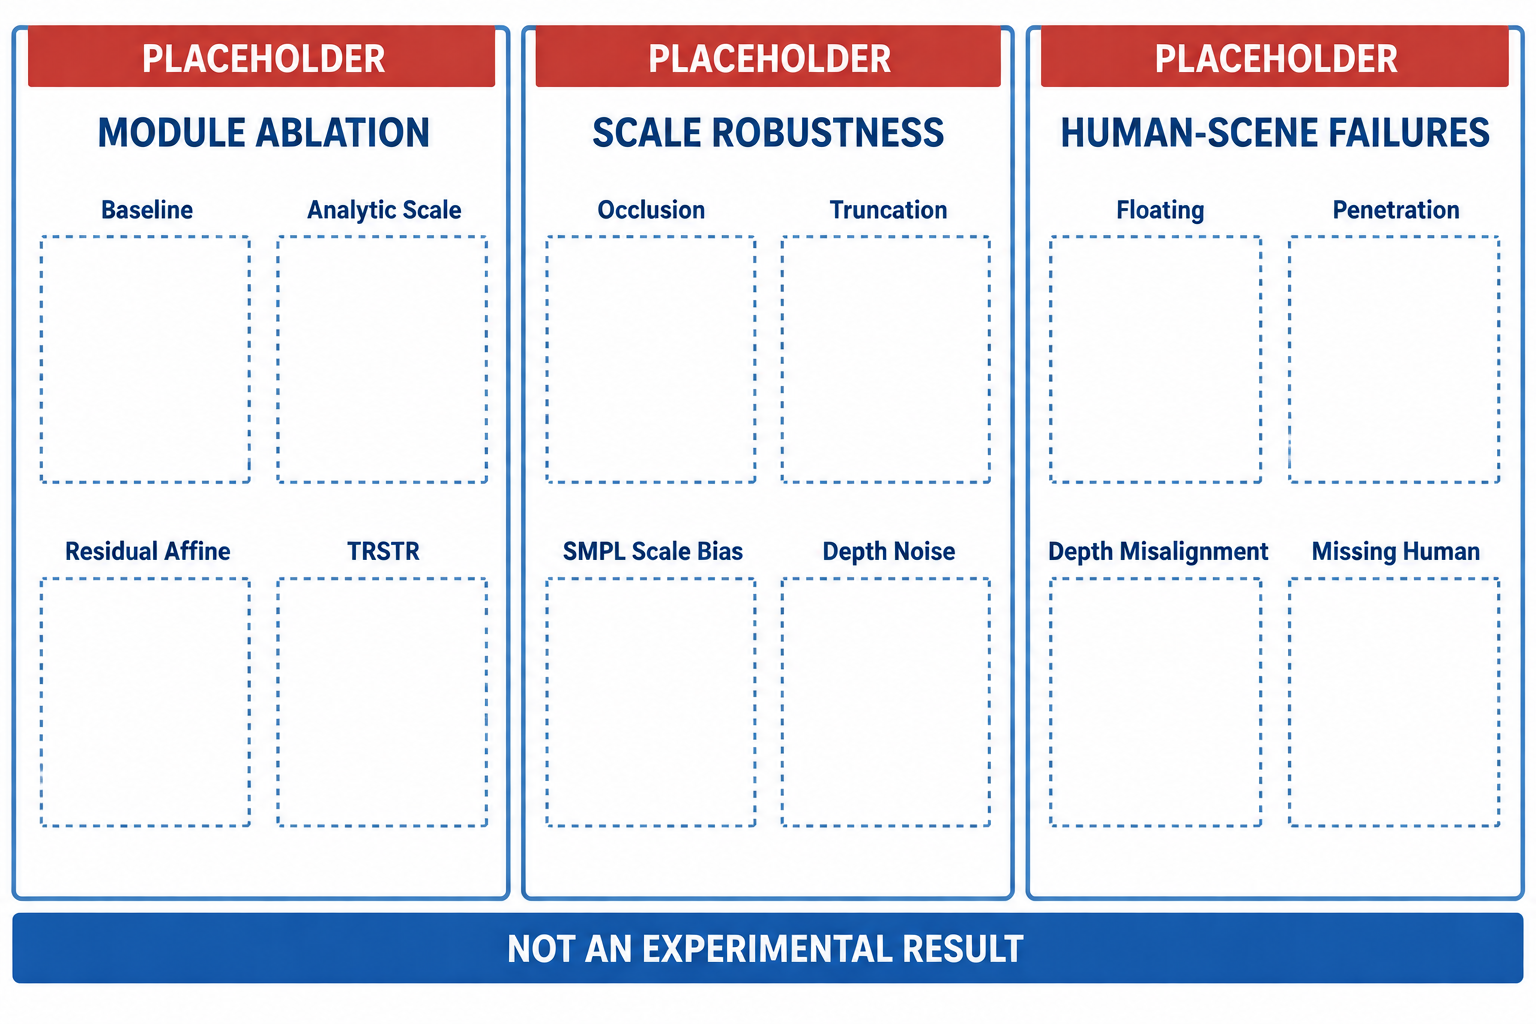
\includegraphics[width=0.96\textwidth]{figures/fig_appendix_placeholder_v2.png}
\caption{\textbf{Appendix experiment placeholder.} This NBAI-generated image previews the intended layout for ablation, robustness, and failure-case results. It is prominently marked as PLACEHOLDER and contains no real samples, values, or experimental conclusions. It must be completely replaced with verified server results in the final version.}
\label{fig:appendix-placeholder}
\end{figure}

The real ablation suite should compare visible front surfaces with root/joint anchors, median with mean aggregation, scale-only, bias-only, and scale-plus-bias calibration, frame-level with clip-level scale, single- with multi-person consensus, and the TRSTR region representation, ray/tangent voting, gates, uncertainty, person gate, and iteration count. It should also include zero-residual and shuffled-conditioning counterfactuals and a numerical pose/shape invariance check.

\section{TRSTR Refinement, Robustness, and Sensitivity}
\label{app:robustness}

\begin{table}[H]
\caption{Robustness experiment placeholder. The bins and perturbation ranges define the experimental design and do not represent completed results.}
\label{tab:robustness-placeholder}
\centering
\small
\resizebox{\textwidth}{!}{%
\begin{tabular}{lllcccc}
\toprule
Factor & Bin/perturbation & Main issue & W-MPJPE & RTE & Abs Rel & $\delta<1.25$ \\
\midrule
Visible human area & small/medium/large & anchor support & \todoresult & \todoresult & \todoresult & \todoresult \\
Occlusion/truncation & low/medium/high & front-surface validity & \todoresult & \todoresult & \todoresult & \todoresult \\
SMPL scale perturbation & $\pm5/10/15\%$ & metric-prior bias & \todoresult & \todoresult & \todoresult & \todoresult \\
Number of people & 1/2/$\geq3$ & multi-person consensus & \todoresult & \todoresult & \todoresult & \todoresult \\
Frames without a human & 0--100\% & scale fallback & \todoresult & \todoresult & \todoresult & \todoresult \\
Relative-depth noise & controlled perturbation & upstream propagation & \todoresult & \todoresult & \todoresult & \todoresult \\
\bottomrule
\end{tabular}
}
\end{table}

Errors in real human dimensions or SMPL shape directly affect absolute scale and are therefore the most important robustness risk for GroundedHuman. The final version must report this experiment; ordinary successful qualitative examples are not a substitute.

\section{Efficiency, Parameters, and Scalability}
\label{app:efficiency}

\begin{table}[H]
\caption{Placeholder for efficiency and resource usage. Test conditions and values require server measurements.}
\label{tab:efficiency-placeholder}
\centering
\small
\begin{tabular}{lccc}
\toprule
Module & Time & Peak memory & Parameters \\
\midrule
VGGT-Ω & \todoresult & \todoresult & frozen \\
NLF & \todoresult & \todoresult & frozen \\
Front-surface scale & \todoresult & \todoresult & 0 \\
HSI residual affine & \todoresult & \todoresult & \todoresult \\
TRSTR & \todoresult & \todoresult & \todoresult \\
End-to-end & \todoresult & \todoresult & \todoresult \\
\bottomrule
\end{tabular}
\end{table}

Final measurements must fix the GPU, input resolution, clip length, and number of people, and state whether data loading, human detection, visualization, and disk I/O are included. A quality--runtime trade-off for the number of TRSTR iterations should also be reported.

\section{Additional Qualitative Results, Failure Cases, and Responsible Use}
\label{app:limitations}

The contents corresponding to Figs.~\ref{fig:temporal-4d}, \ref{fig:general-reconstruction}, and~\ref{fig:metric-measurement} remain in the main paper to present temporal reconstruction, general 3D diagnostics, and interpretable real-world measurements. The final supplementary material should additionally show coarse scale, residual affine calibration, and TRSTR before/after results for the same sequences, together with cases involving occlusion, truncation, mutual occlusion among multiple people, long intervals without a visible human, and upstream depth failure.

The main failure chains include insufficient anchor support caused by invisibility or severe truncation; biased metric priors caused by incorrect SMPL shape or height; unreliable local probes caused by VGGT-Ω relative-structure errors; failed environment/other-human separation under dynamic objects or multi-person occlusion; and the inability of translation-only TRSTR to correct pose, shape, or fine-grained contact.

\placeholdernote{The final version must replace the FAILURE CASES panel in Fig.~\ref{fig:appendix-placeholder} with real failure samples and report detection signals, fallback behavior, and unresolved limitations.}

Human-video reconstruction may be misused for privacy-sensitive behavioral analysis or surveillance. This work is limited to geometric reconstruction and does not perform identity recognition or sensitive-attribute inference. Canonical human dimensions may also produce systematic scale bias for children, uncommon body types, or populations outside the training distribution; this issue must be quantified through the real sensitivity experiments in Appendix~\ref{app:robustness}.


\end{document}
